\documentclass[10pt,a4paper]{article}
\usepackage[utf8]{inputenc}
\usepackage{amsmath}
\usepackage{amsfonts}
\usepackage{amssymb}
\usepackage{graphicx}
\usepackage{geometry}
\usepackage{fancyhdr}
\usepackage{listings}
\usepackage{xcolor}
\usepackage{float}
\usepackage{subcaption}
\usepackage{url}

% Page geometry
\geometry{left=2cm,right=2cm,top=2cm,bottom=2cm}

% Header and footer
\pagestyle{fancy}
\fancyhf{}
\fancyhead[L]{EN3160 - Assignment 1}
\fancyhead[R]{220148G - Eashan S.G.S}
\fancyfoot[C]{\thepage}

% Code listing style
\lstset{
    language=Python,
    basicstyle=\tiny\ttfamily,
    keywordstyle=\color{blue},
    commentstyle=\color{green},
    stringstyle=\color{red},
    numbers=left,
    numberstyle=\tiny,
    stepnumber=1,
    numbersep=5pt,
    backgroundcolor=\color{gray!10},
    frame=single,
    breaklines=true,
    breakatwhitespace=true,
    tabsize=2
}

\begin{document}

% Title page
\begin{titlepage}
    \centering
    \vspace*{2cm}

    
\includegraphics[width=6cm]{image.png}\\[1cm]
    {\LARGE Department of Electronic and Telecommunications Engineering}\\[0.5cm]
    
    {\Large EN3160 Image Processing and Machine Vision}\\[1cm]
    
    {\huge \textbf{Intensity Transformations and Neighborhood Filtering}}\\[0.5cm]
    {\Large Assignment 1}\\[2cm]
    
    {\Large Eashan S.G.S ( 220148G )}\\[1cm]
    
    \vfill
    
    {\large \today}
\end{titlepage}

\section*{GitHub Repository}
Link to GitHub repository: \url{https://github.com/sahas-eashan/EN3160-Assignment-1}

\section{Question 1}
The given intensity transformation can be realized using piecewise linear segments. The transformation enhances mid-intensity pixels while keeping low and high intensity pixels relatively unchanged.

\begin{lstlisting}[caption=Intensity transformation implementation]
import cv2 as cv
import numpy as np
import matplotlib.pyplot as plt

# Define piecewise transformation function
c = np.array([(50, 50), (150, 255)], dtype=np.uint8)
t1 = np.linspace(0, 50, 51, dtype=np.uint8)
t2 = np.linspace(100, 255, 150 - 50, dtype=np.uint8)
t3 = np.linspace(150, 255, 256 - 150, dtype=np.uint8)

# Concatenate all segments to create the transformation array
lut = np.concatenate((t1, t2, t3), axis=0)
lut = lut[:256]

\end{lstlisting}

\begin{figure}[H]
    \centering
    \begin{subfigure}{0.45\textwidth}
        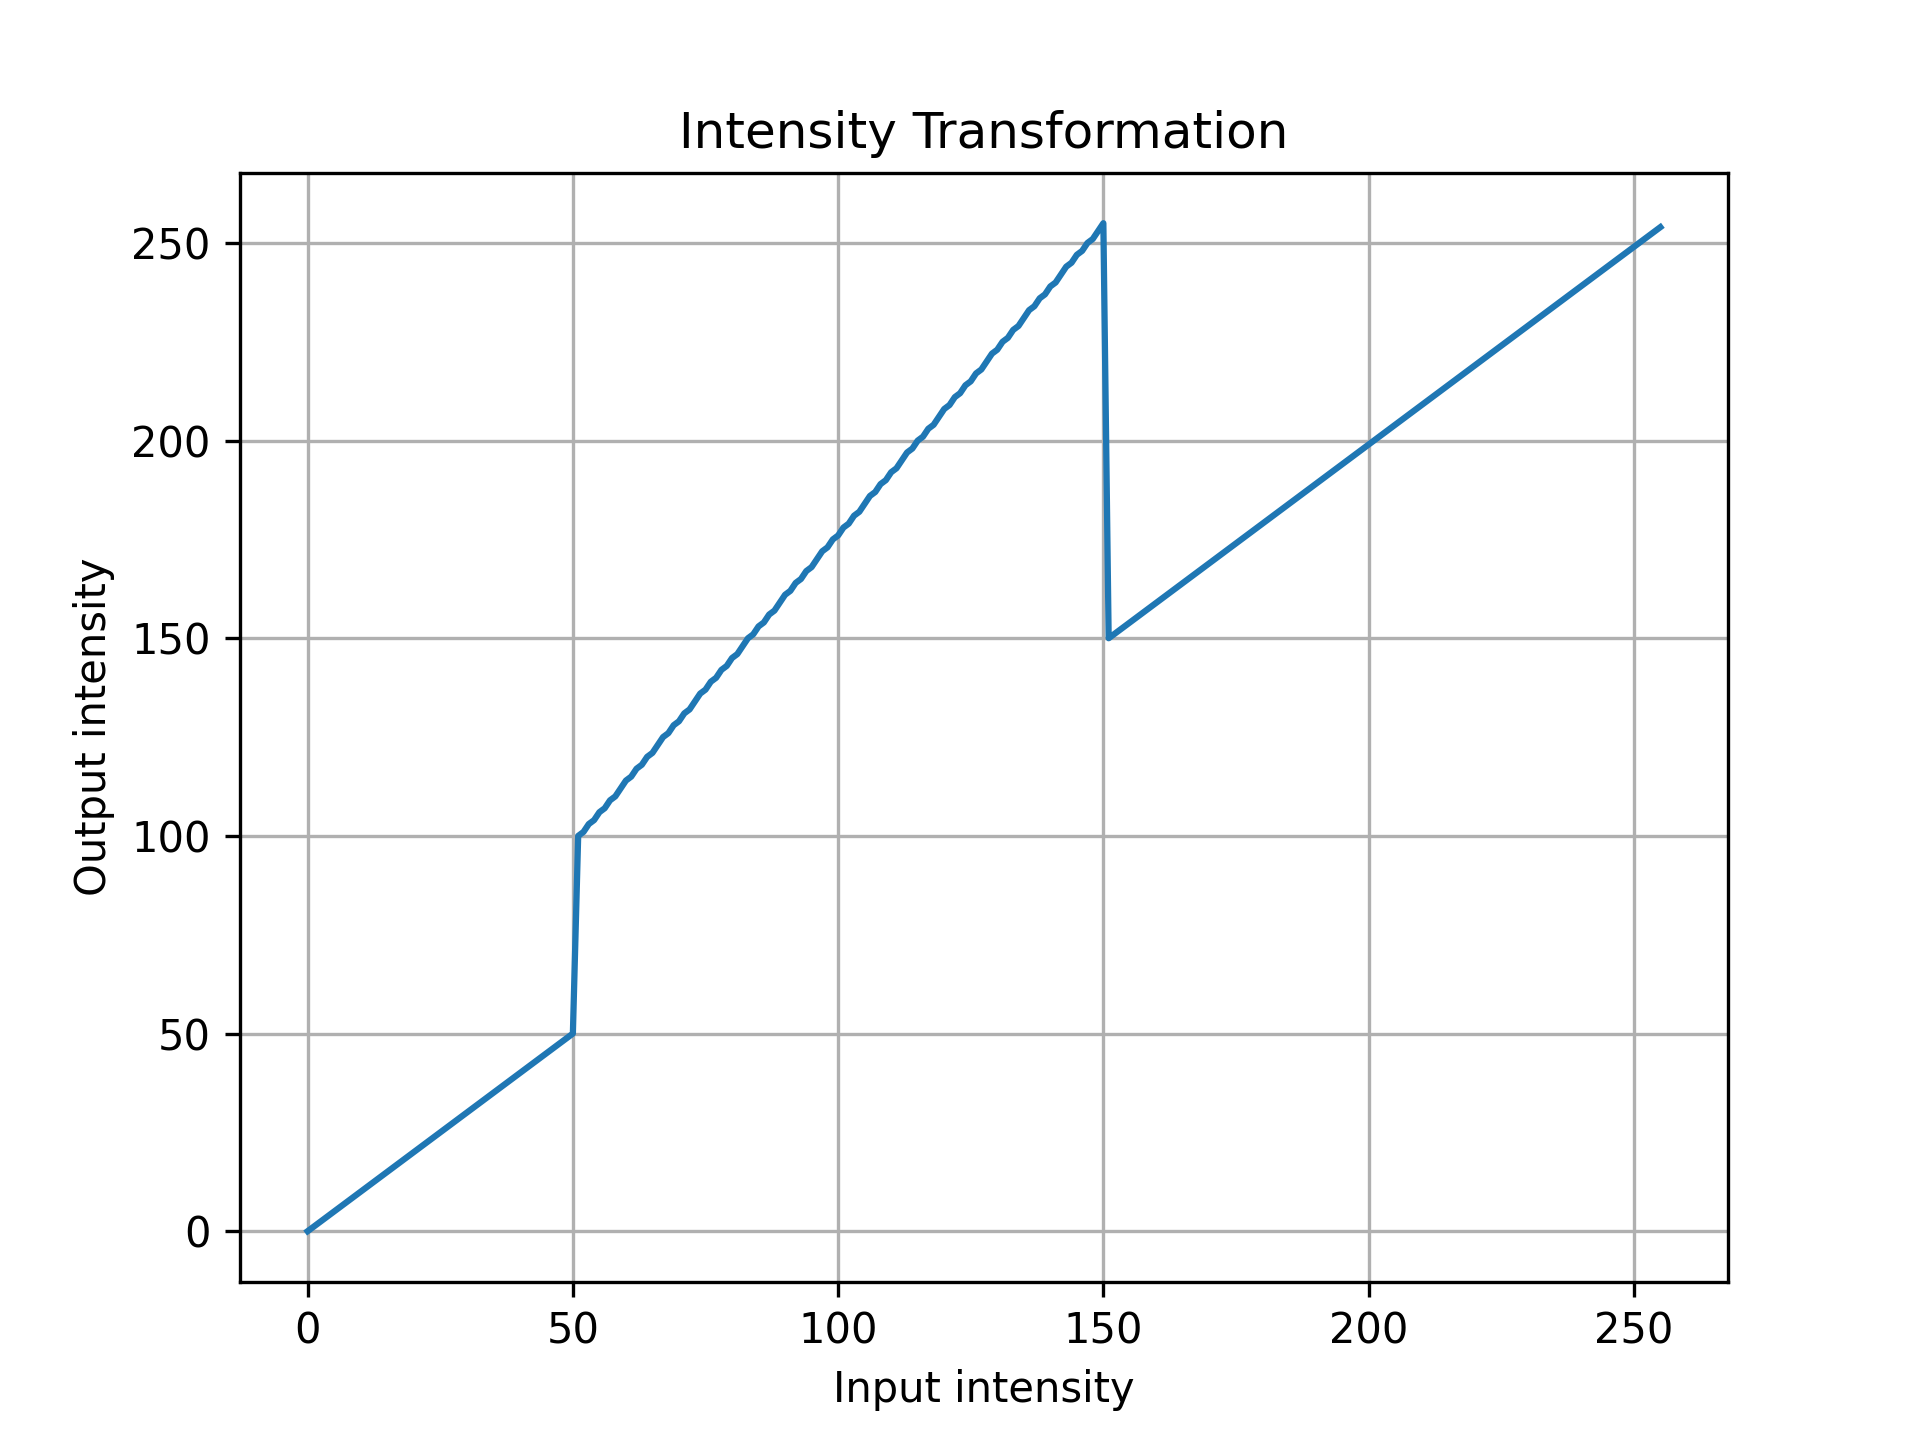
\includegraphics[width=\textwidth]{task1/transformation_curve.png}
        \caption{Intensity transformation curve}
    \end{subfigure}
    \hfill
    \begin{subfigure}{0.25\textwidth}
        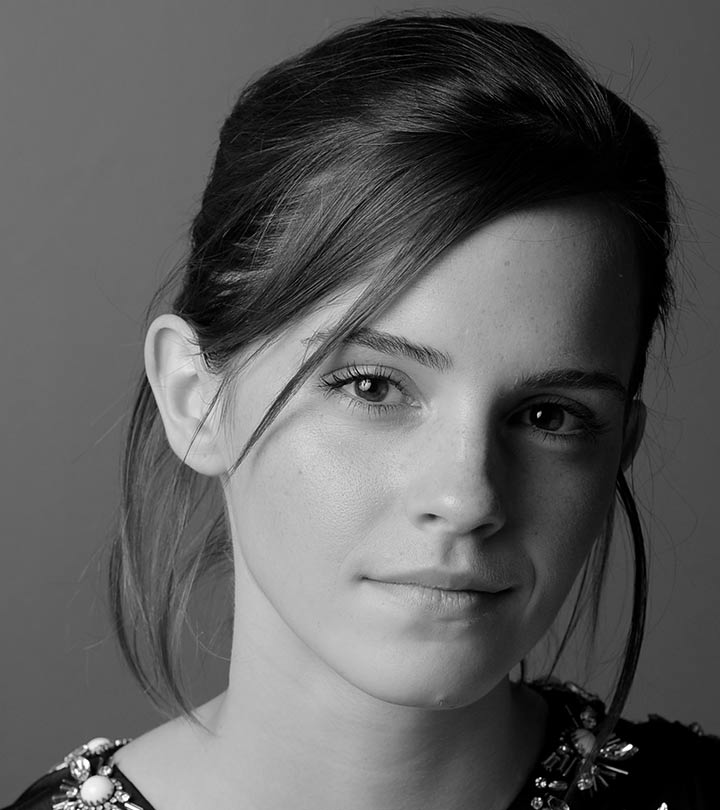
\includegraphics[width=\textwidth]{task1/original.png}
        \caption{Original image}
    \end{subfigure}
    \begin{subfigure}{0.25\textwidth}
        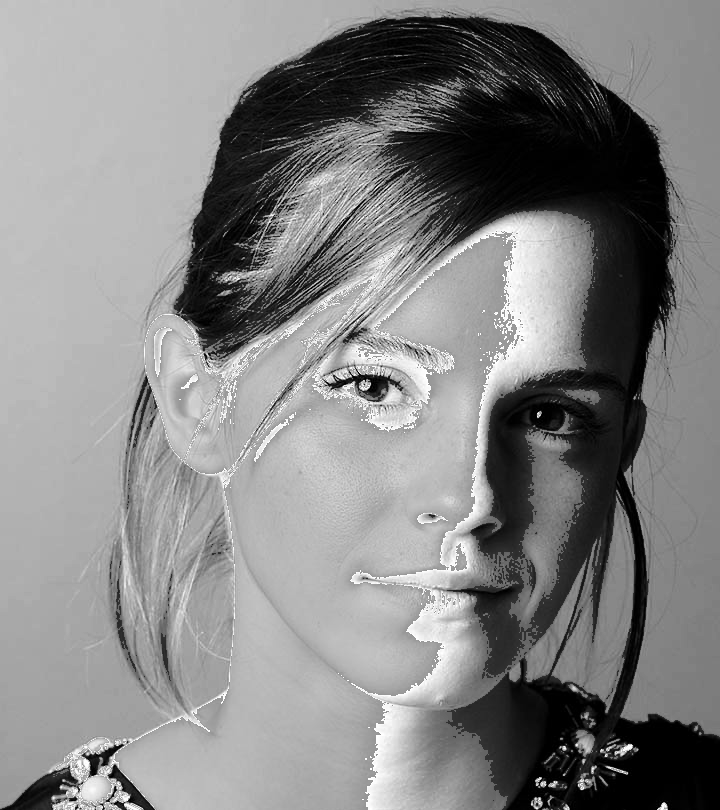
\includegraphics[width=\textwidth]{task1/transformed.png}
        \caption{transformed image}
    \end{subfigure}
    \caption{Intensity transformation results for Question 1}
\end{figure}

\textbf{Interpretation:} The transformation creates jump discontinuities that result in high contrast regions. Mid-intensity pixels are enhanced while preserving the extreme intensity values.

\section{Question 2}
To accentuate white and gray matter in the brain MRI, I used Gaussian pulse transformations centered at different intensity values to highlight specific tissue types.

\begin{lstlisting}[caption=Brain tissue enhancement]
# White matter enhancement (centered around intensity 150)
mu_white, sigma_white = 200, 20
lut_white = (
    (255 * np.exp(-((x - mu_white) ** 2) / (2 * sigma_white**2)))
    .clip(0, 255)
    .astype(np.uint8)
)

# Gray matter enhancement (centered around intensity 200)
mu_gray, sigma_gray = 140, 20
lut_gray = (
    (255 * np.exp(-((x - mu_gray) ** 2) / (2 * sigma_gray**2)))
    .clip(0, 255)
    .astype(np.uint8)
)
\end{lstlisting}

\begin{figure}[H]
    \centering
    \begin{subfigure}{0.24\textwidth}
        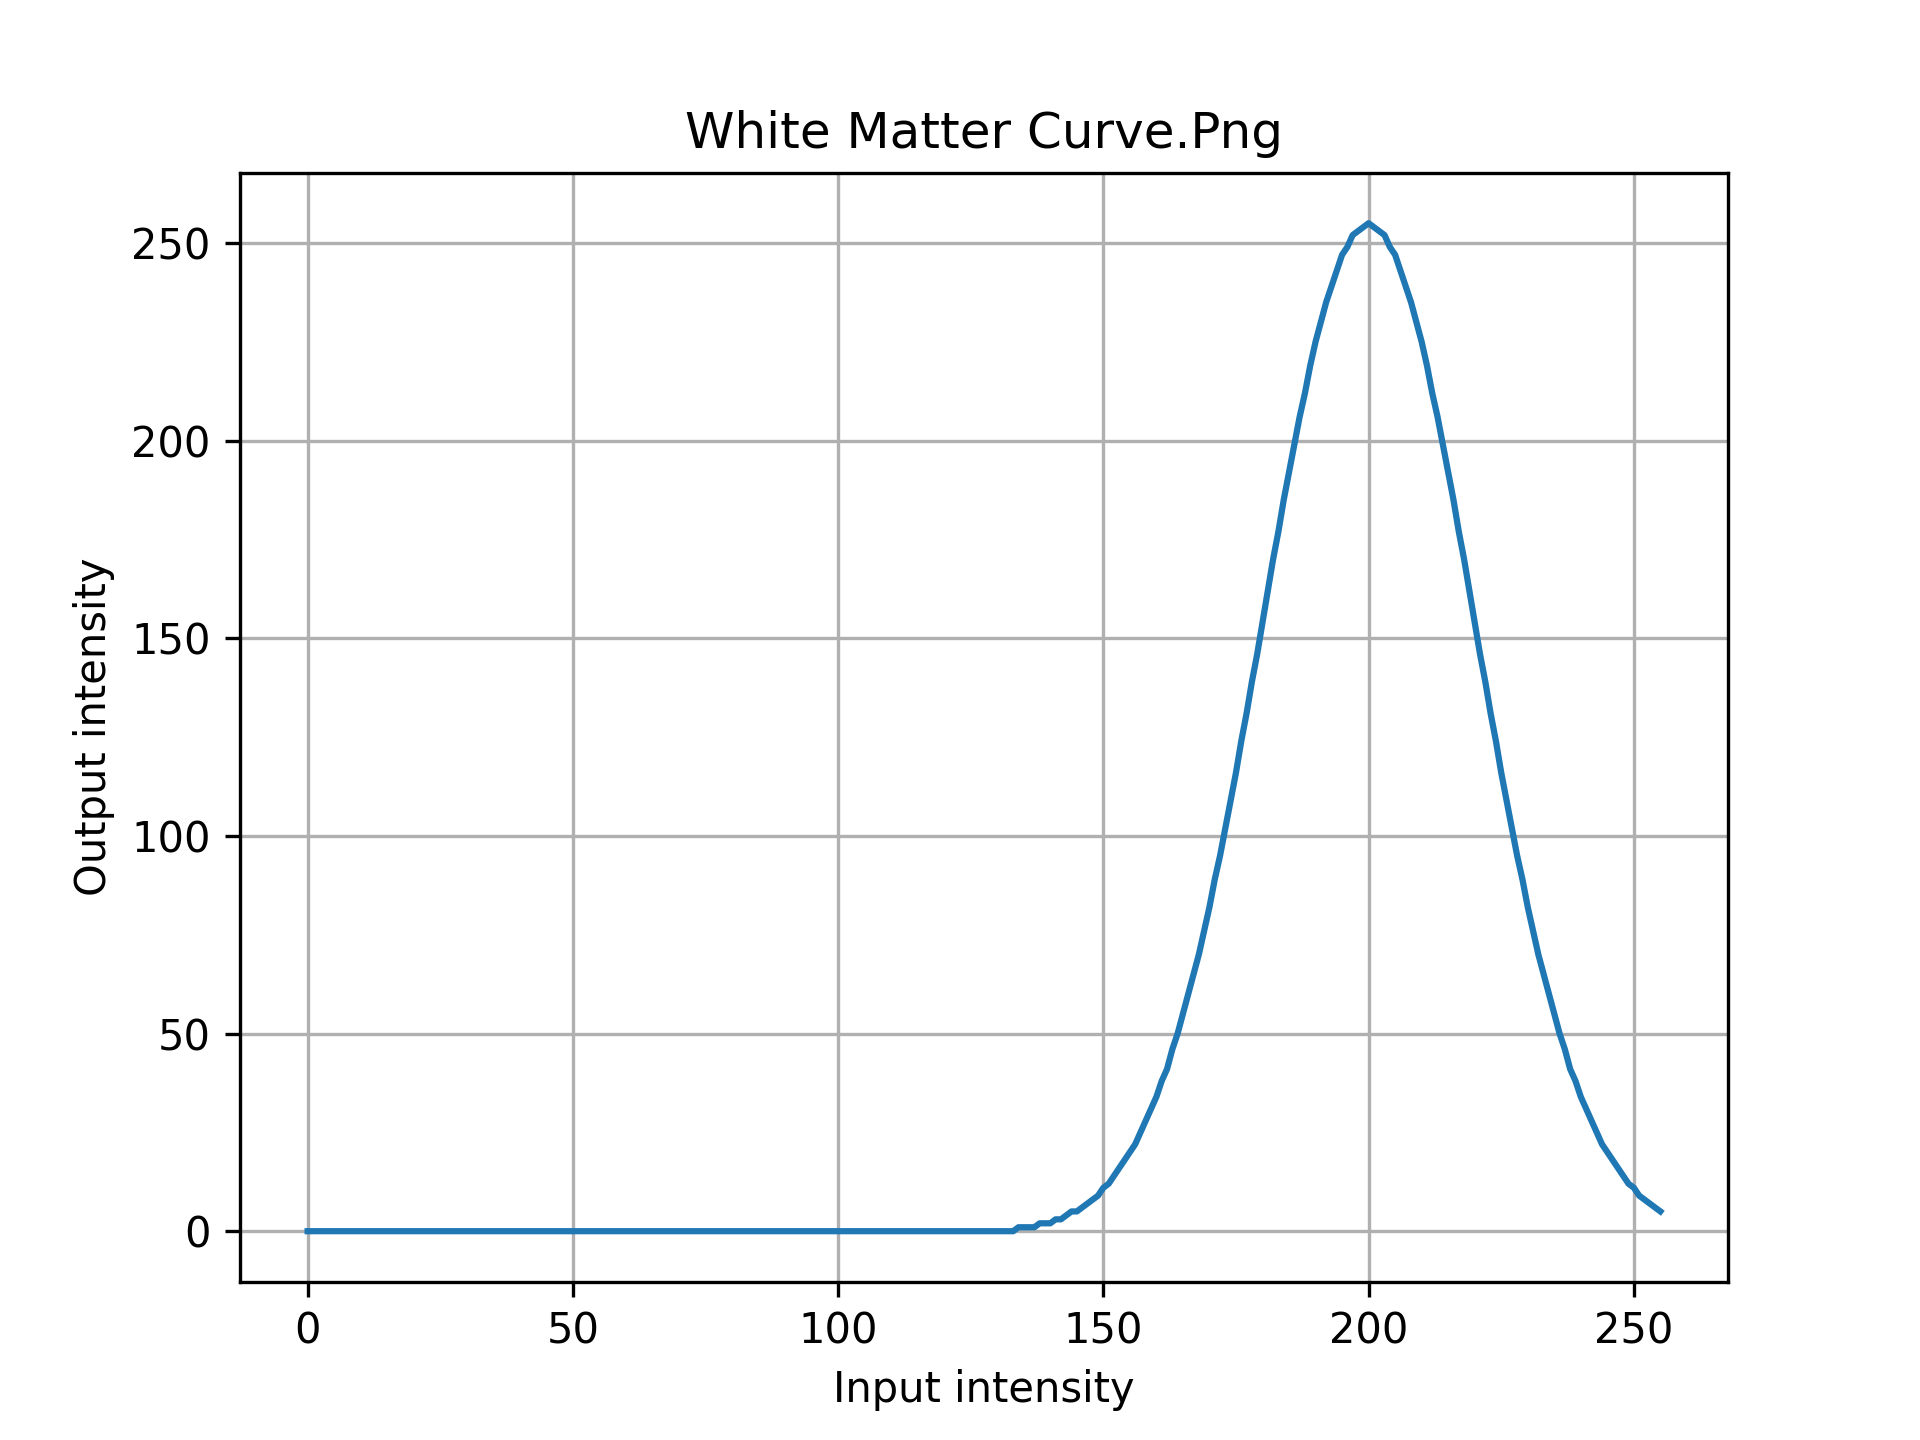
\includegraphics[width=\textwidth]{task2/white_matter_curve.png}
        \caption{White matter curve}
    \end{subfigure}
    \begin{subfigure}{0.24\textwidth}
        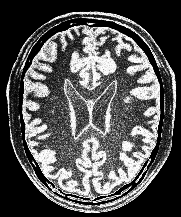
\includegraphics[width=\textwidth]{task2/white_matter.png}
        \caption{White matter enhanced}
    \end{subfigure}
    \begin{subfigure}{0.24\textwidth}
        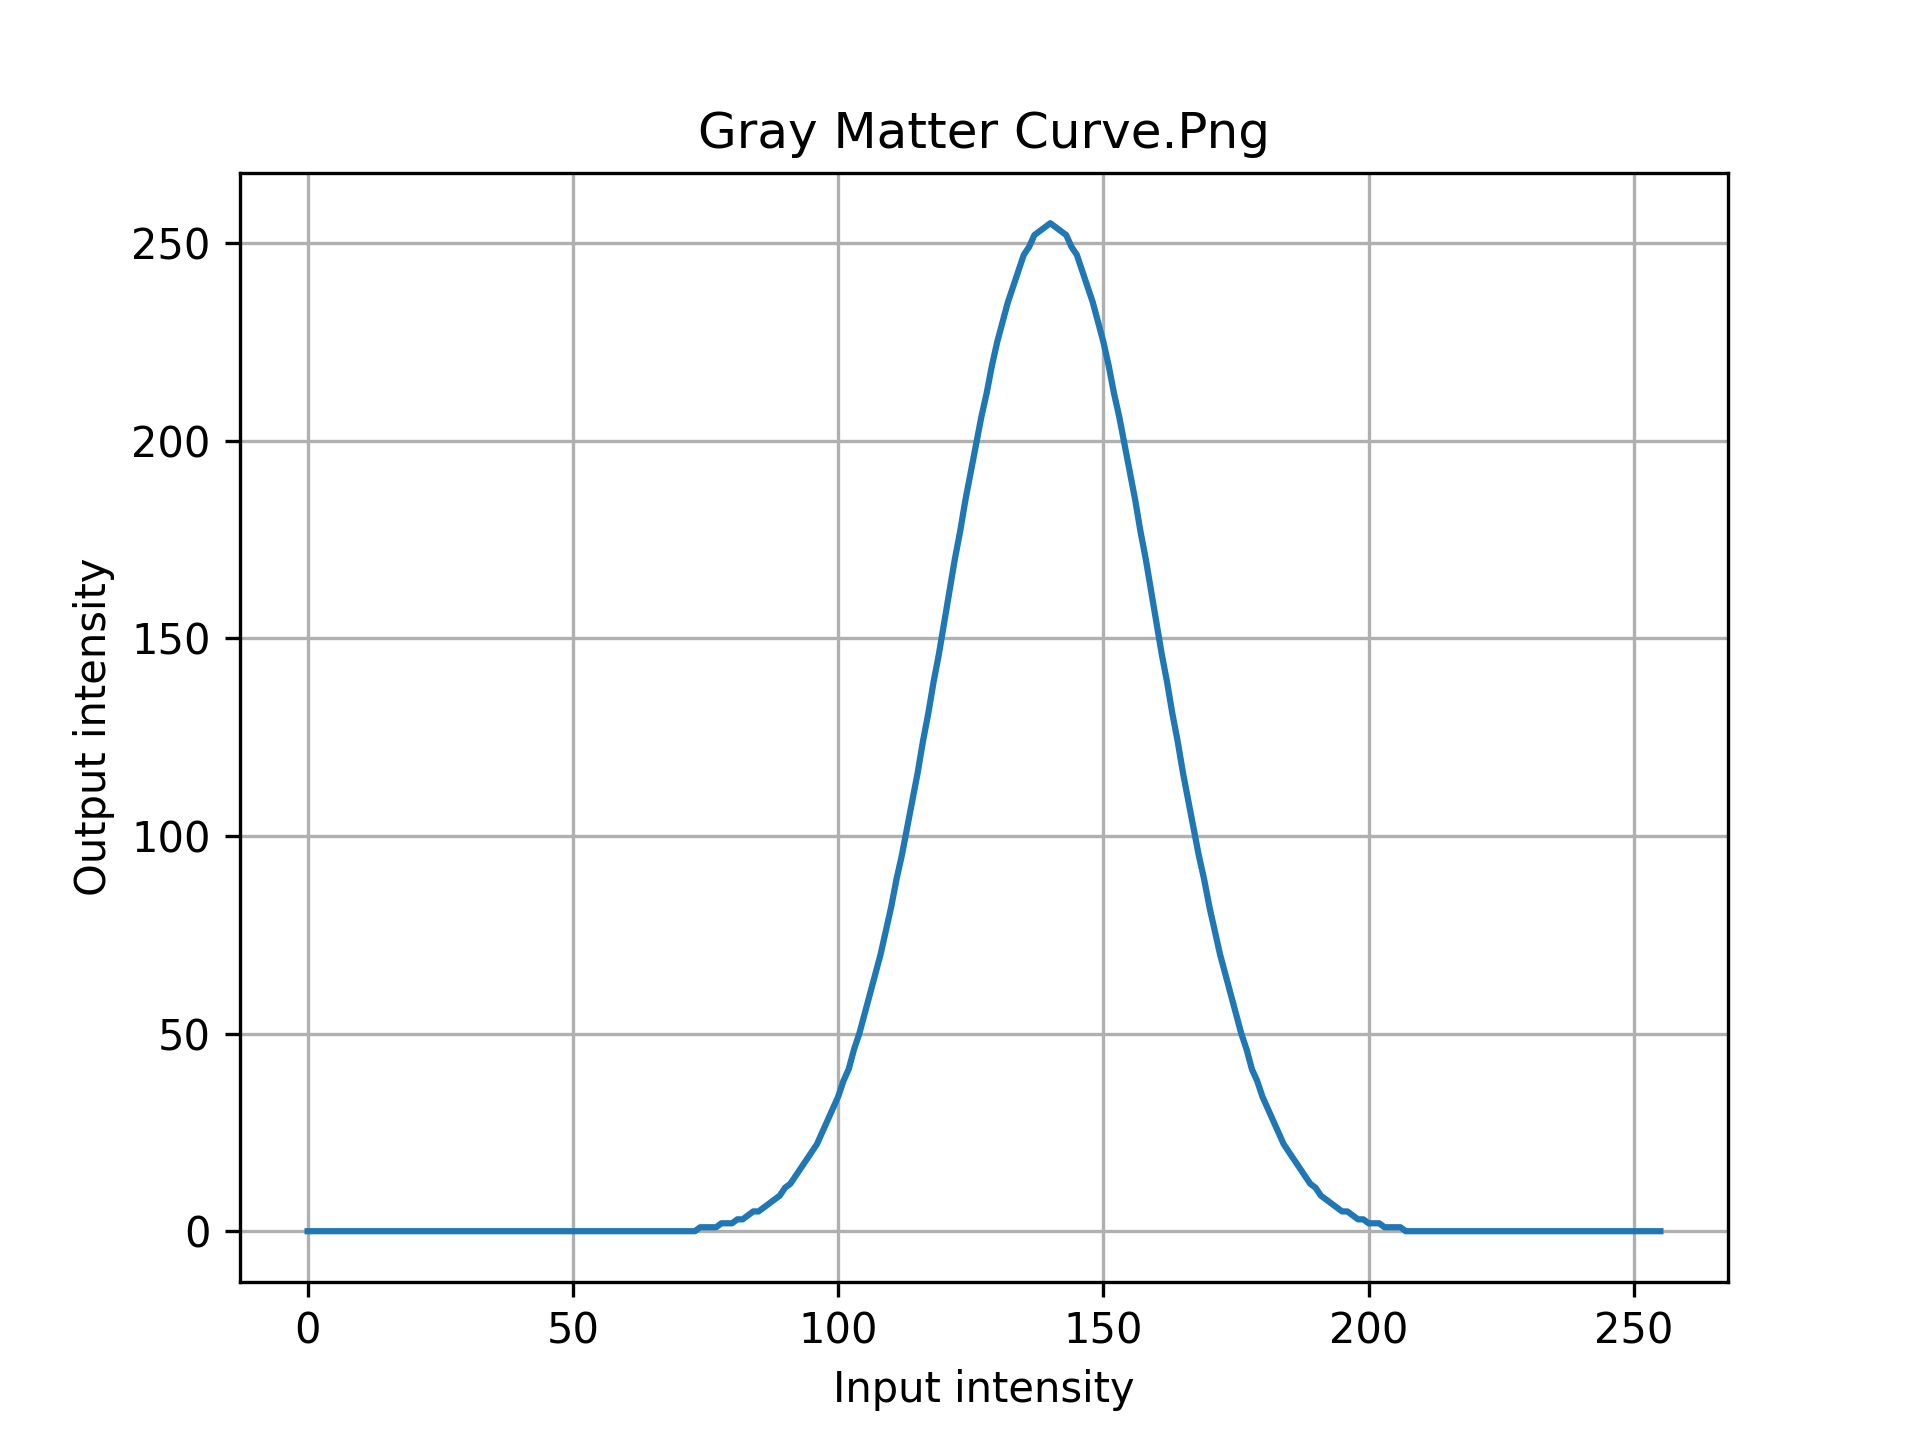
\includegraphics[width=\textwidth]{task2/gray_matter_curve.png}
        \caption{Gray matter curve}
    \end{subfigure}
    \begin{subfigure}{0.24\textwidth}
        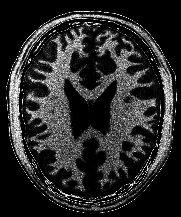
\includegraphics[width=\textwidth]{task2/gray_matter.png}
        \caption{Gray matter enhanced}
    \end{subfigure}
    \caption{Brain tissue enhancement results}
\end{figure}

\textbf{Interpretation:} The Gaussian pulse transformations provide smooth contrast enhancement for specific intensity ranges, effectively highlighting white and gray matter tissues.

\section{Question 3}
Gamma correction was applied to the L* channel of the L*a*b* color space to adjust image lightness and improve shadow details.

\begin{lstlisting}[caption=Gamma correction implementation]
# Convert to L*a*b* color space
lab = cv.cvtColor(img, cv.COLOR_BGR2Lab)
L, a, b = cv.split(lab)

# Apply gamma correction (gamma = 0.5)
gamma = 0.5
L_corrected = np.clip((L / 255.0) ** gamma * 255, 0, 255).astype(np.uint8)

# Merge channels back
lab_corrected = cv.merge((L_corrected, a, b))
img_corrected = cv.cvtColor(lab_corrected, cv.COLOR_Lab2BGR)

\end{lstlisting}

\begin{figure}[H]
    \centering
    \begin{subfigure}{0.48\textwidth}
        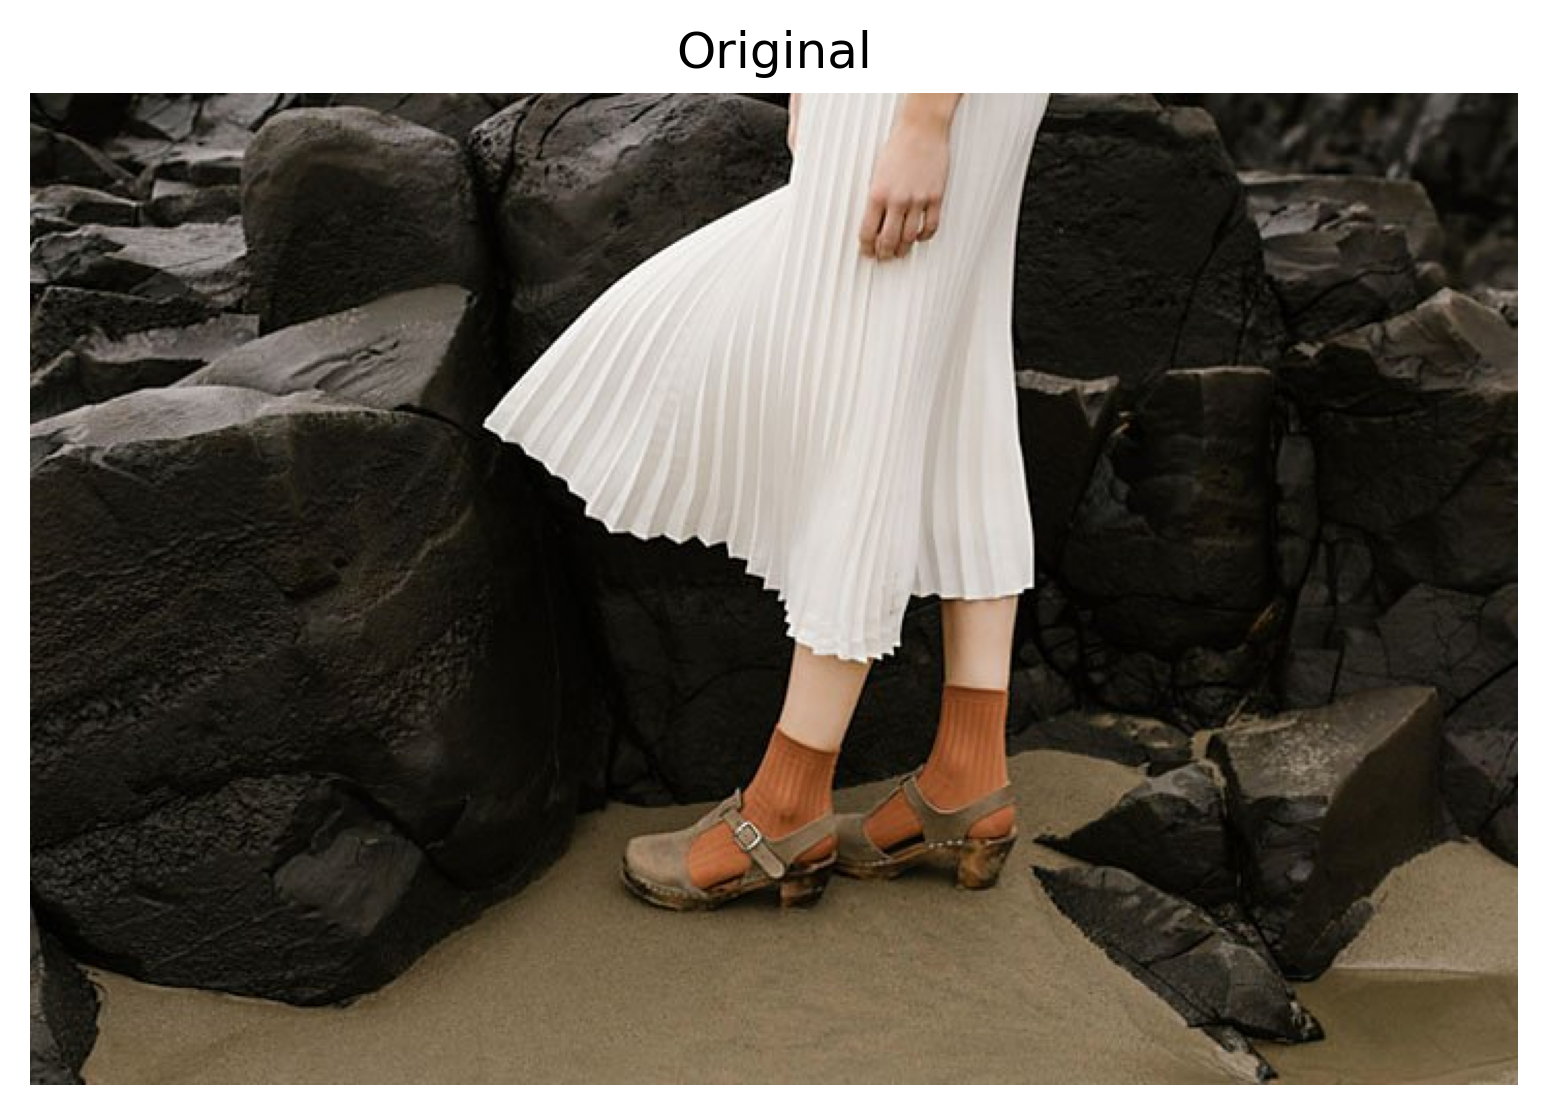
\includegraphics[width=\textwidth]{task3/original_image.png}
        \caption{Original image}
    \end{subfigure}
    \begin{subfigure}{0.48\textwidth}
        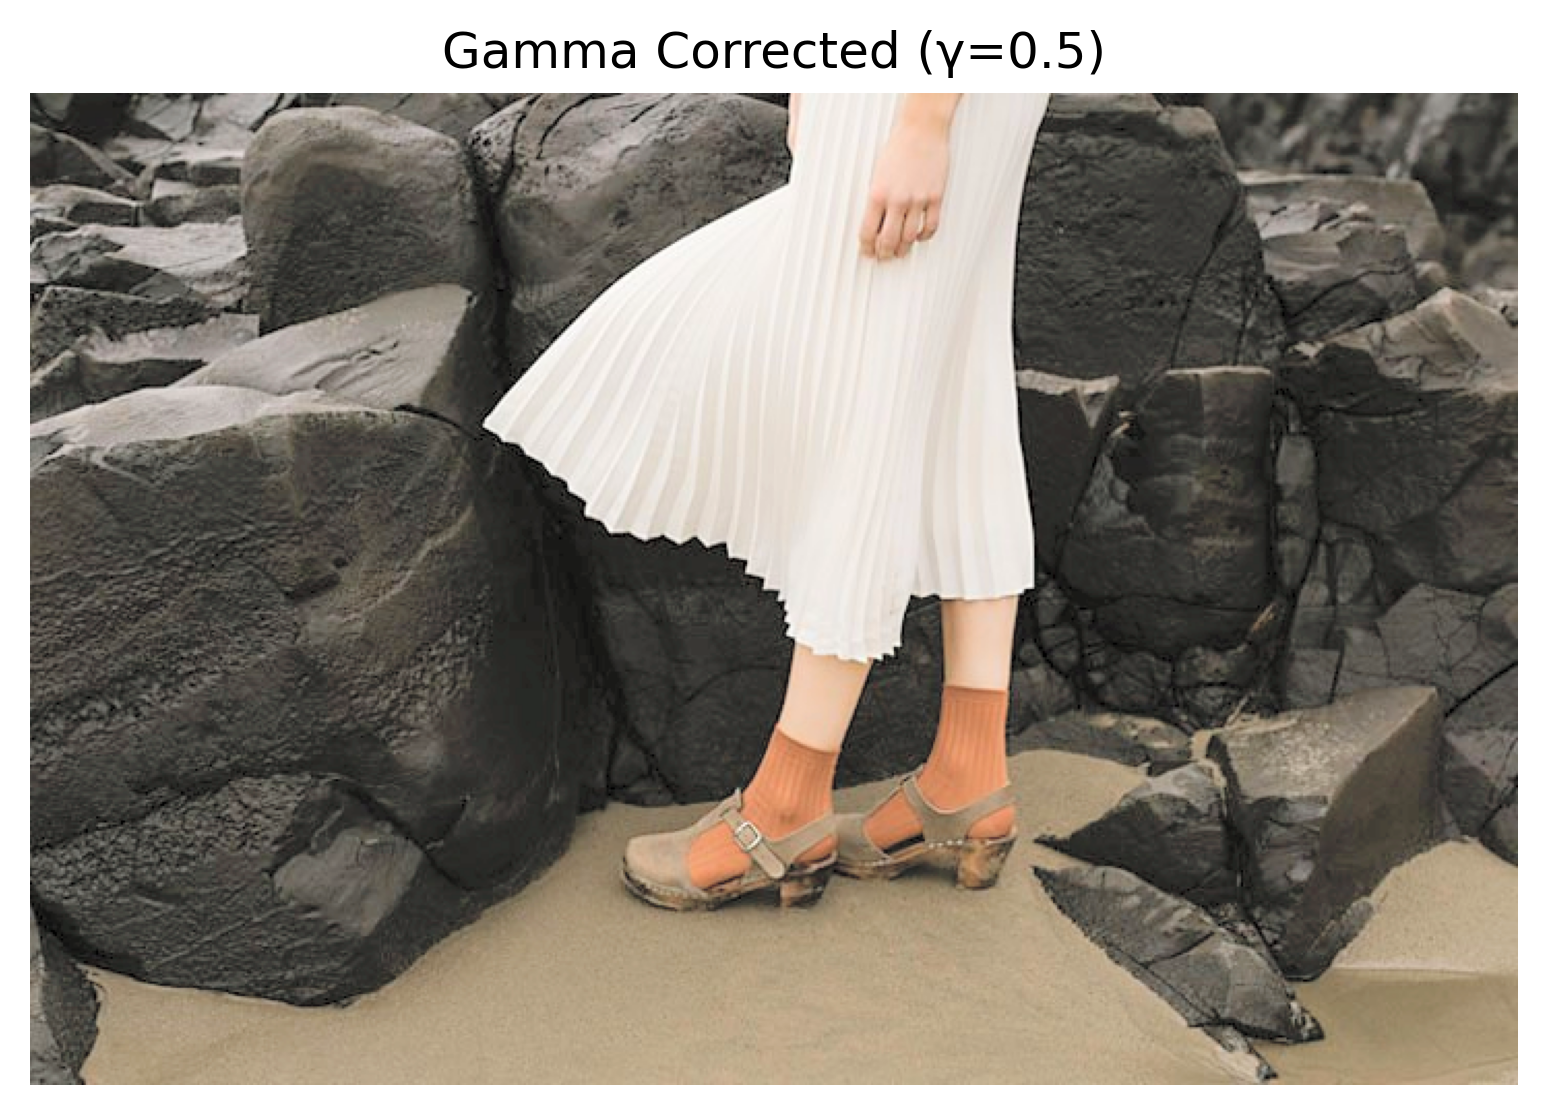
\includegraphics[width=\textwidth]{task3/gamma_corrected_image.png}
        \caption{Gamma corrected image}
    \end{subfigure}
    \hfill
    \caption{Gamma correction results (gamma = 0.5)}
\end{figure}

\begin{figure}[htbp] % avoid forcing [H] unless really needed
  \centering
  \begin{subfigure}[t]{.24\linewidth}\centering
    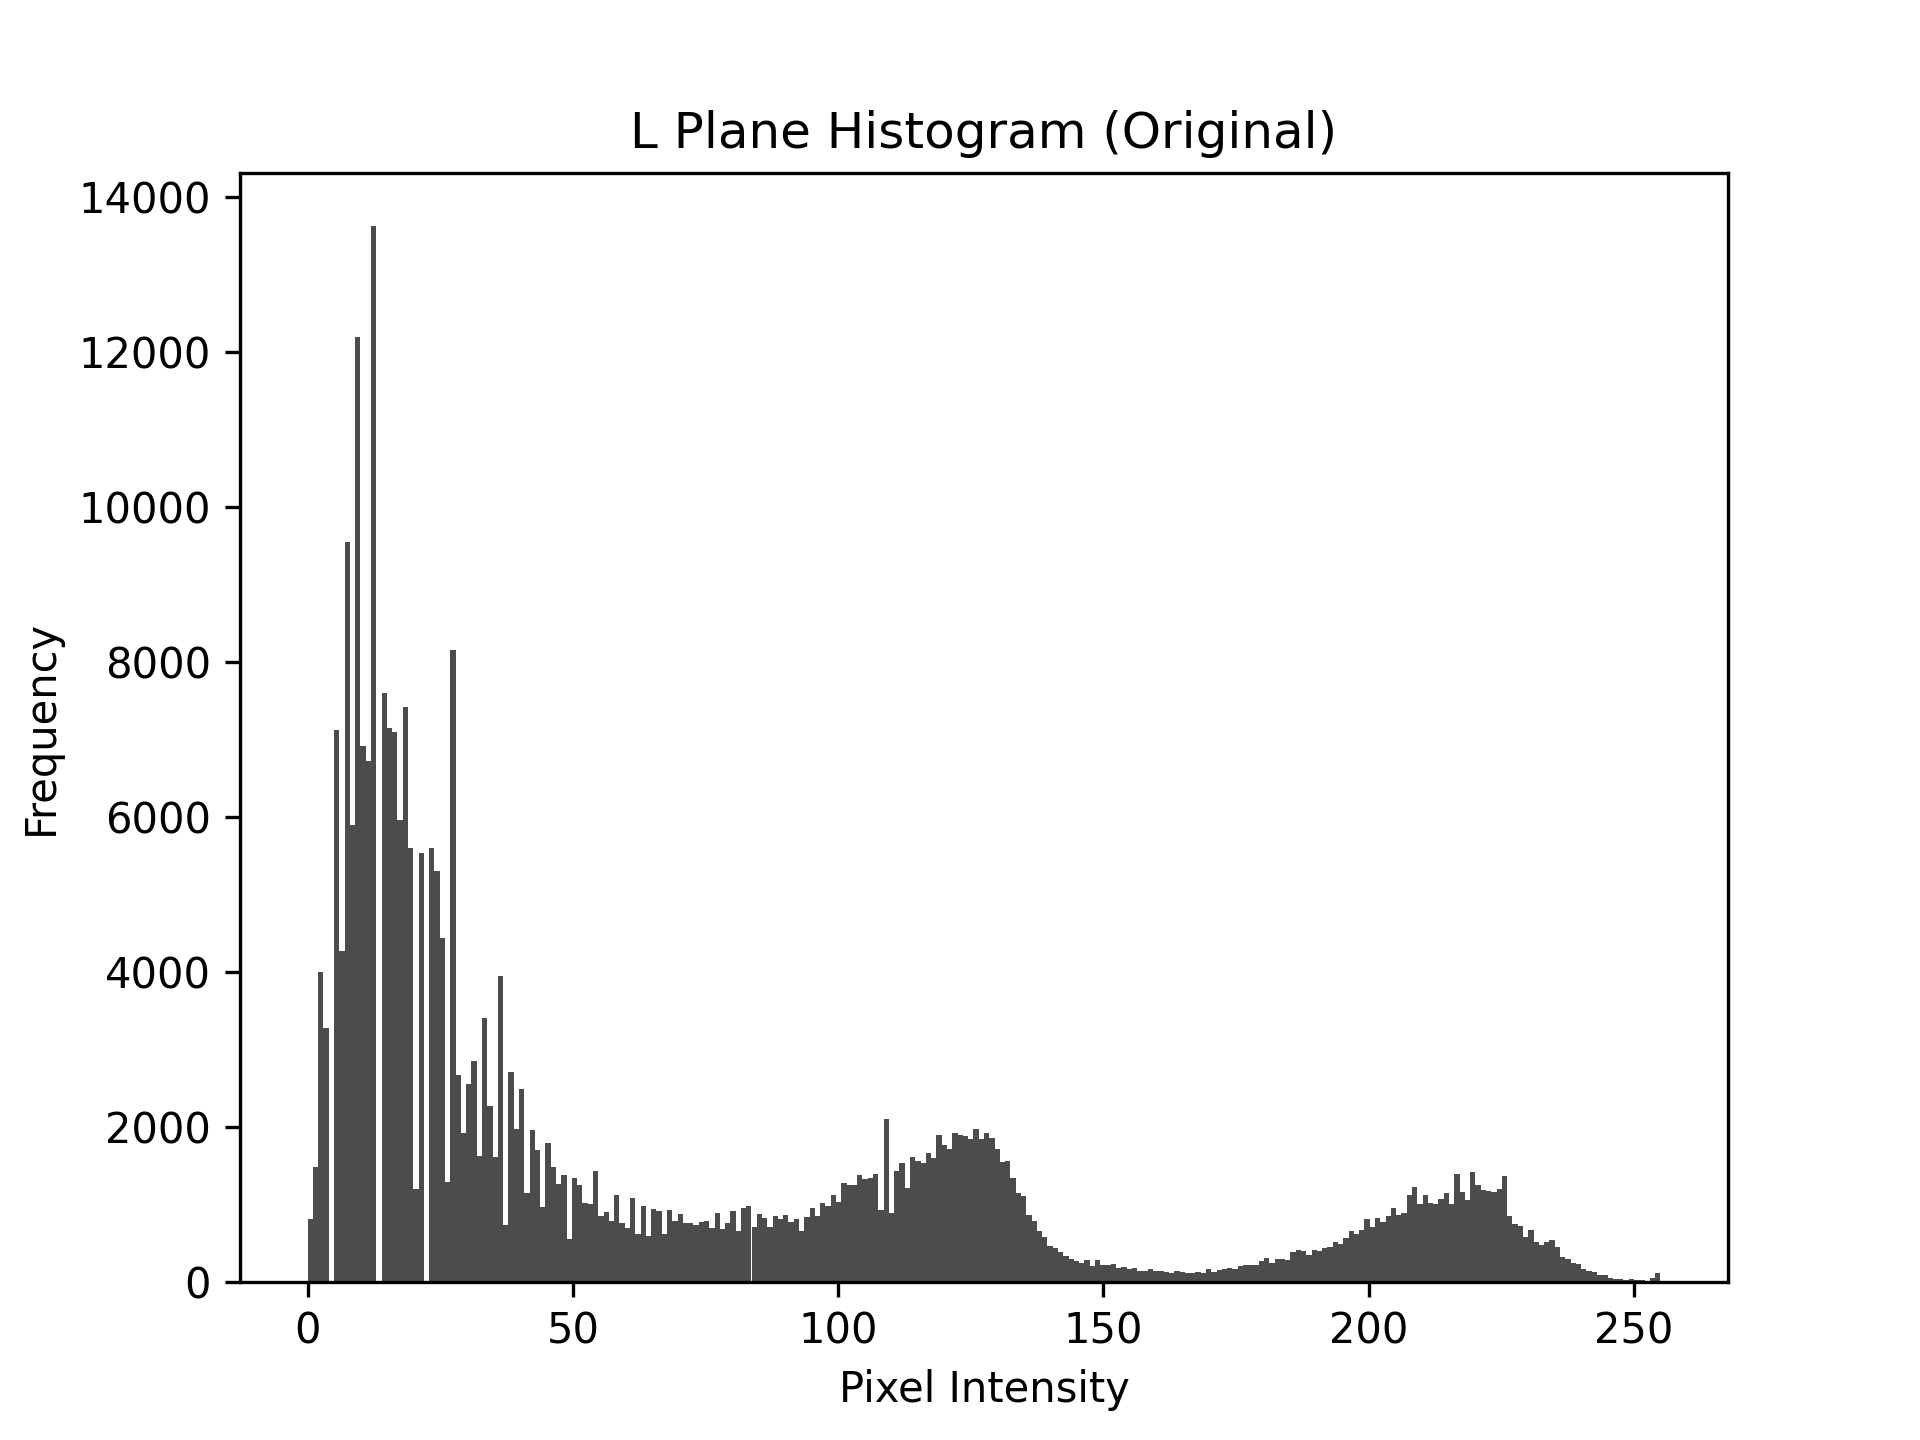
\includegraphics[width=\linewidth]{task3/L_plane_histogram_original.png}
    \caption{L* channel histogram (original)}
  \end{subfigure}\hfill
  \begin{subfigure}[t]{.24\linewidth}\centering
    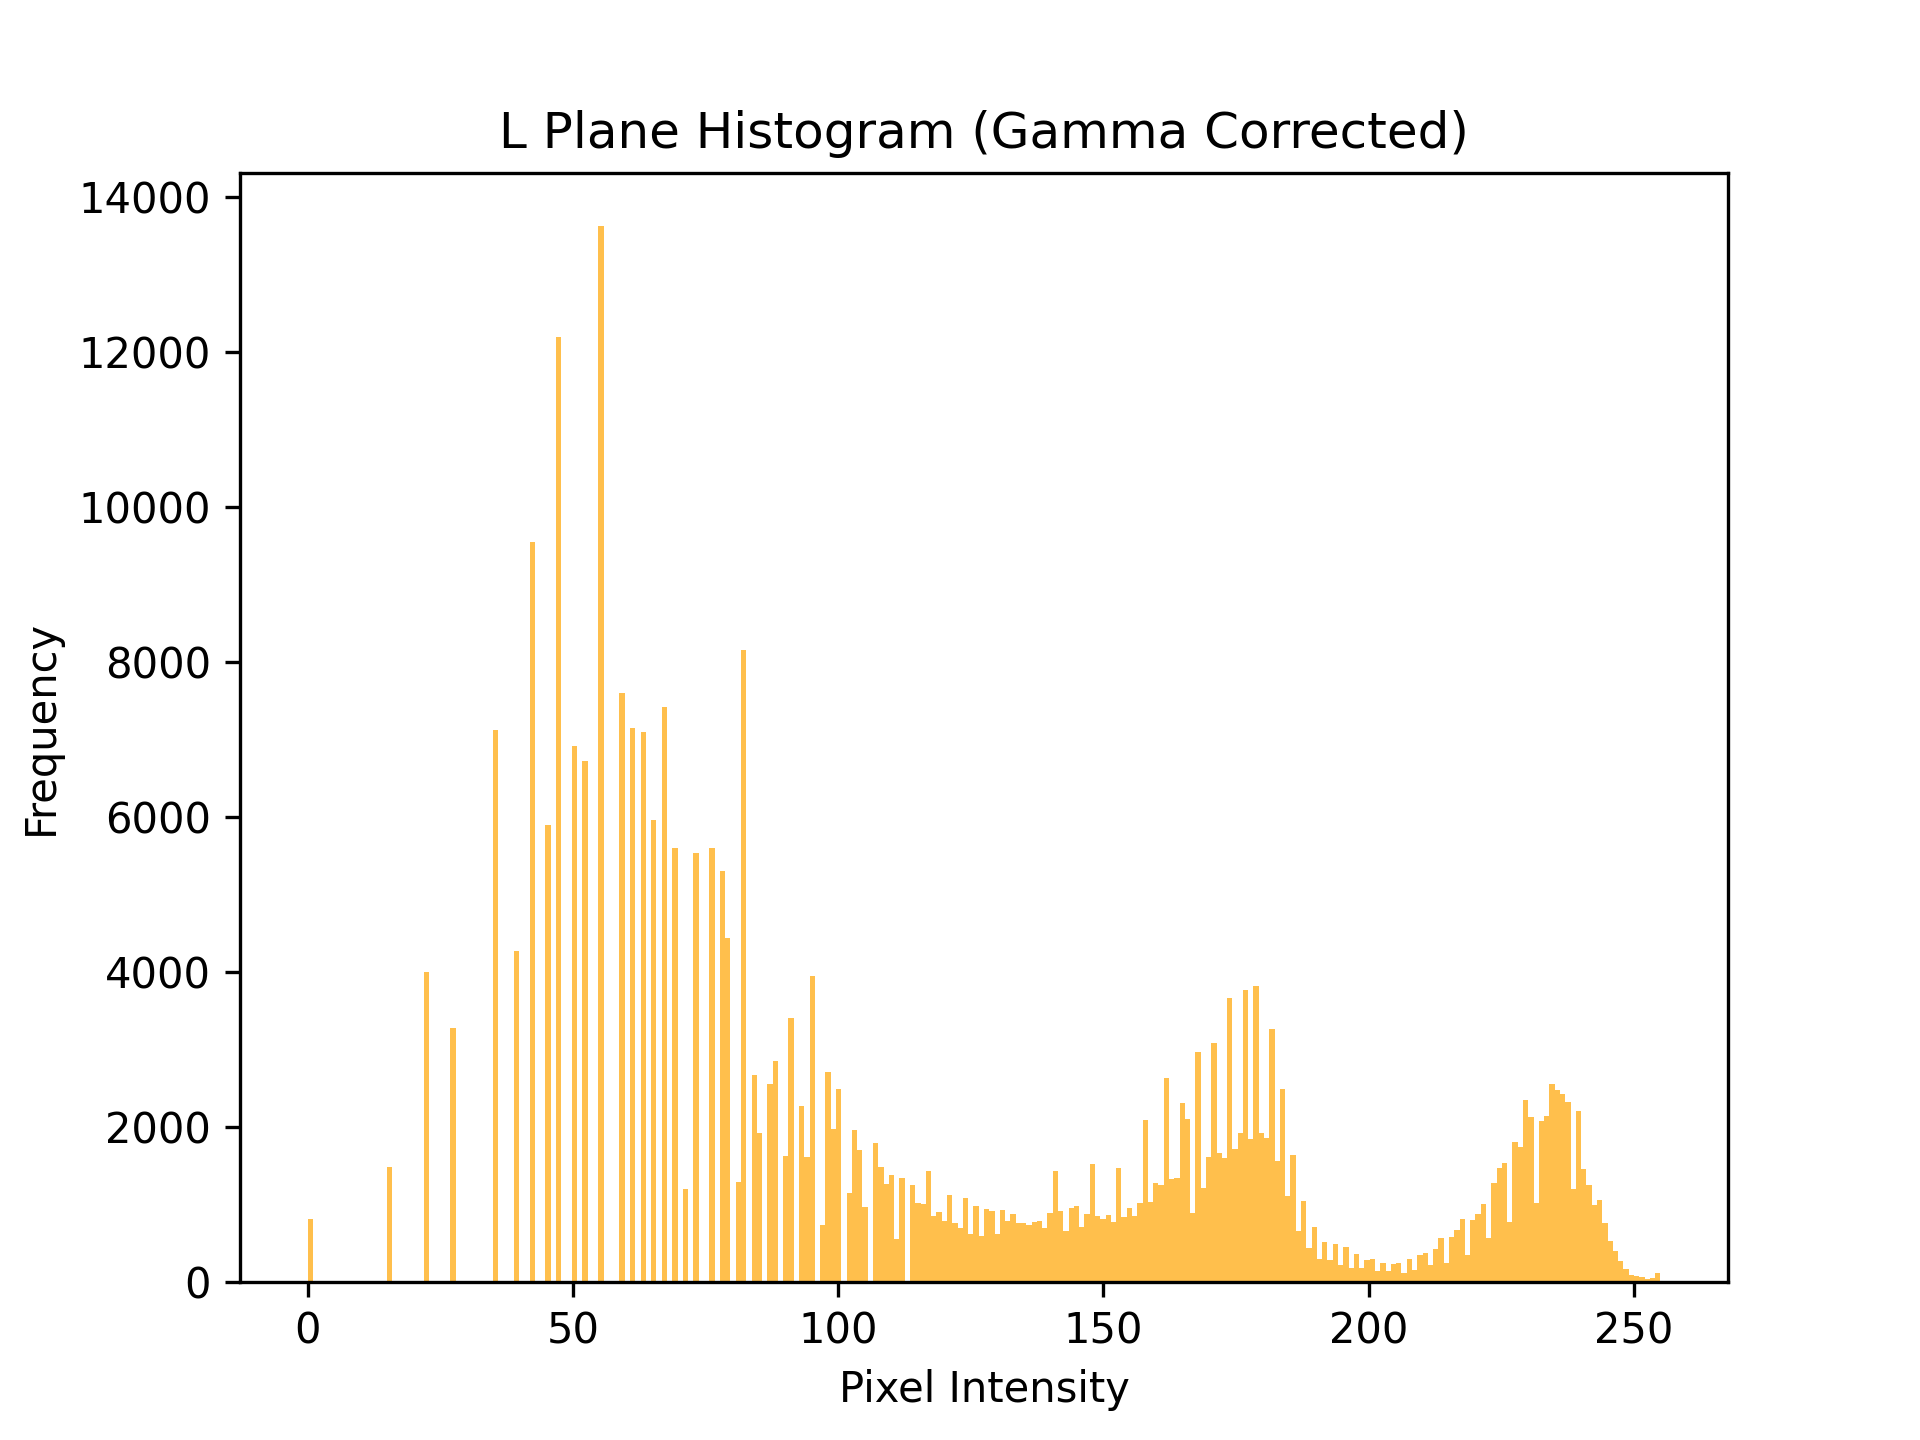
\includegraphics[width=\linewidth]{task3/L_plane_histogram_corrected.png}
    \caption{L* channel histogram (corrected)}
  \end{subfigure}\hfill
  \begin{subfigure}[t]{.24\linewidth}\centering
    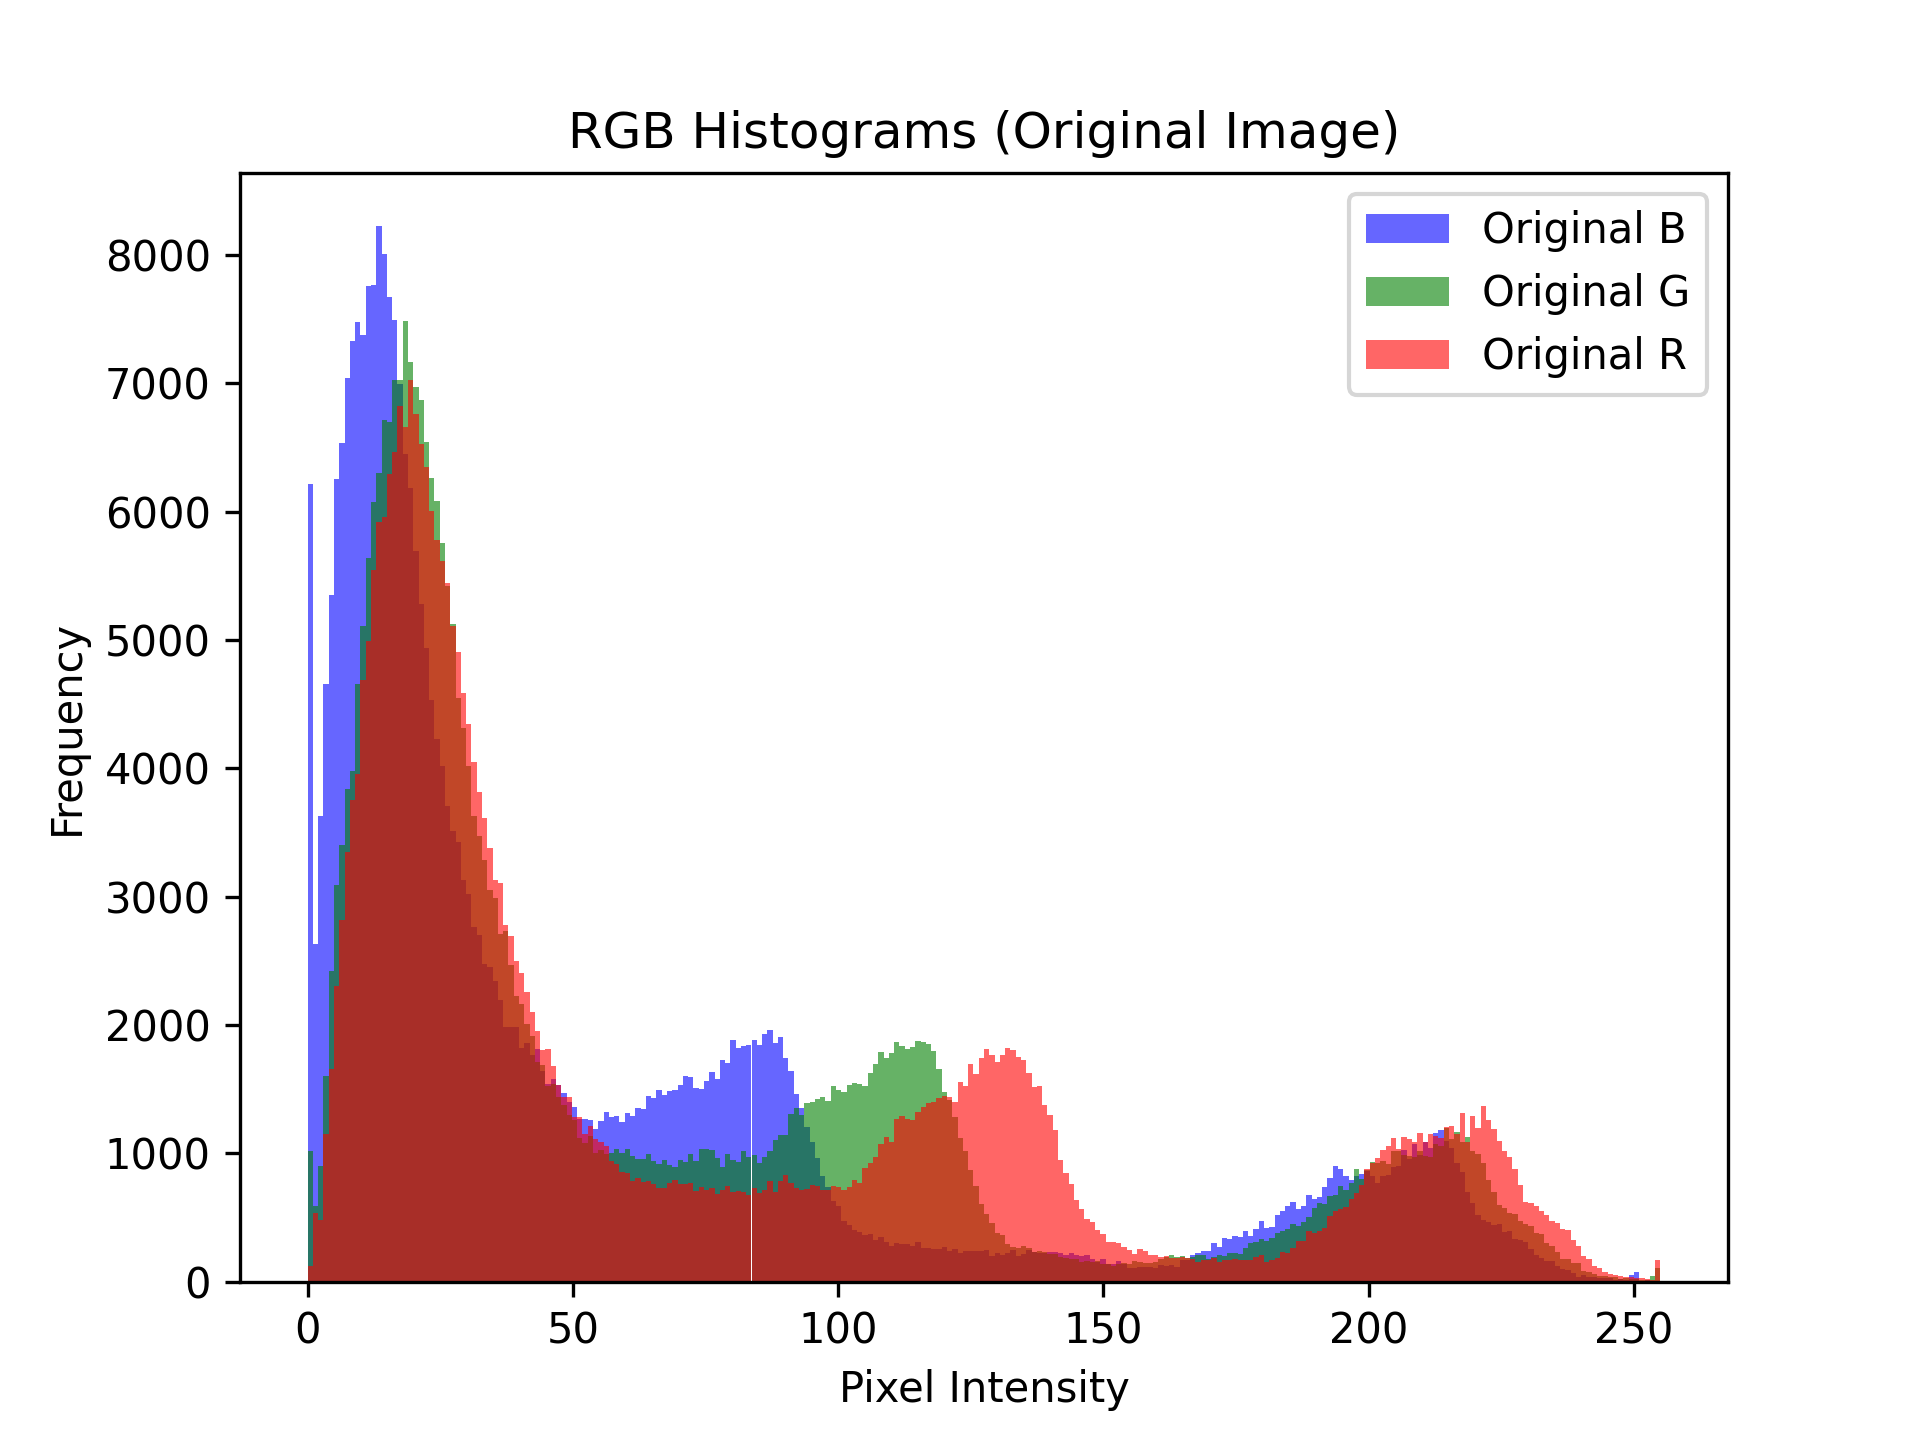
\includegraphics[width=\linewidth]{task3/RGB_histogram_original.png}
    \caption{RGB histogram (original)}
  \end{subfigure}\hfill
  \begin{subfigure}[t]{.24\linewidth}\centering
    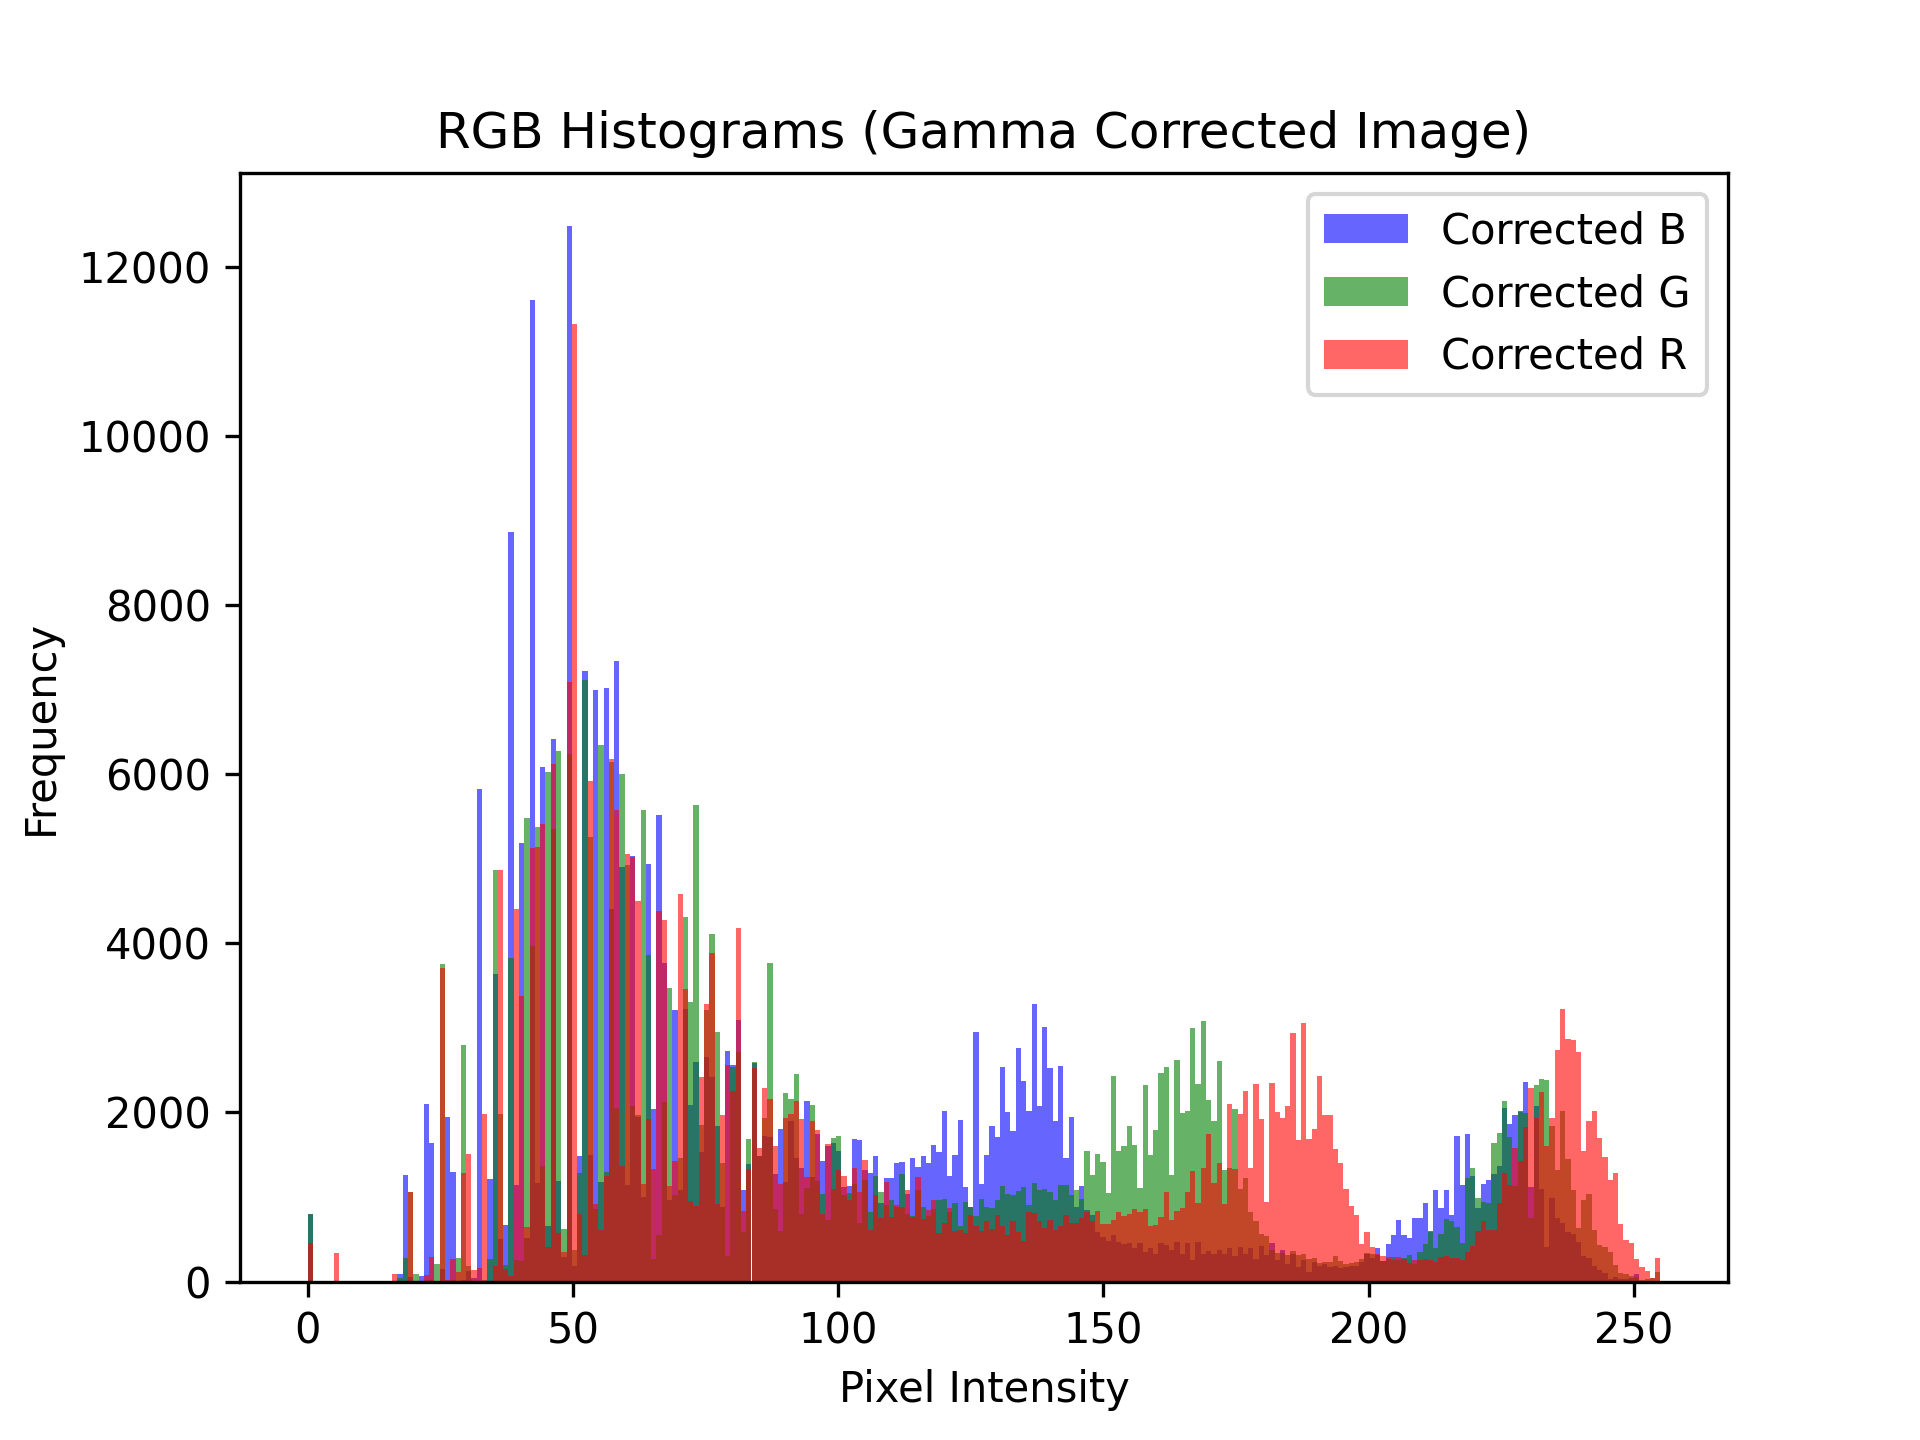
\includegraphics[width=\linewidth]{task3/RGB_histogram_corrected.png}
    \caption{RGB histogram (corrected)}
  \end{subfigure}
  \caption{Histograms of L* and RGB channels (original vs corrected)}
\end{figure}



\textbf{Interpretation:} Gamma correction with gamma = 0.5 lightens the shadows while preserving highlights, improving overall image visibility.

\newpage

\section{Question 4}
The vibrance enhancement was achieved by applying a specific transformation to the saturation channel in HSV color space.

\begin{lstlisting}[caption=Vibrance enhancement]
# Convert to HSV and split channels
hsv = cv.cvtColor(img, cv.COLOR_BGR2HSV)
H, S, V = cv.split(hsv)

# Define vibrance transformation
a = 0.65
sigma = 70.0
x = np.arange(256, dtype=np.float32)
f = x + a * 128.0 * np.exp(-((x - 128.0) ** 2) / (2.0 * sigma**2))
lut = np.clip(f, 0, 255).astype(np.uint8)

# Apply to saturation channel
S_enh = cv.LUT(S, lut)
hsv_enh = cv.merge((H, S_enh, V))
img_enh = cv.cvtColor(hsv_enh, cv.COLOR_HSV2BGR)

\end{lstlisting}

\begin{figure}[H]
    \centering
    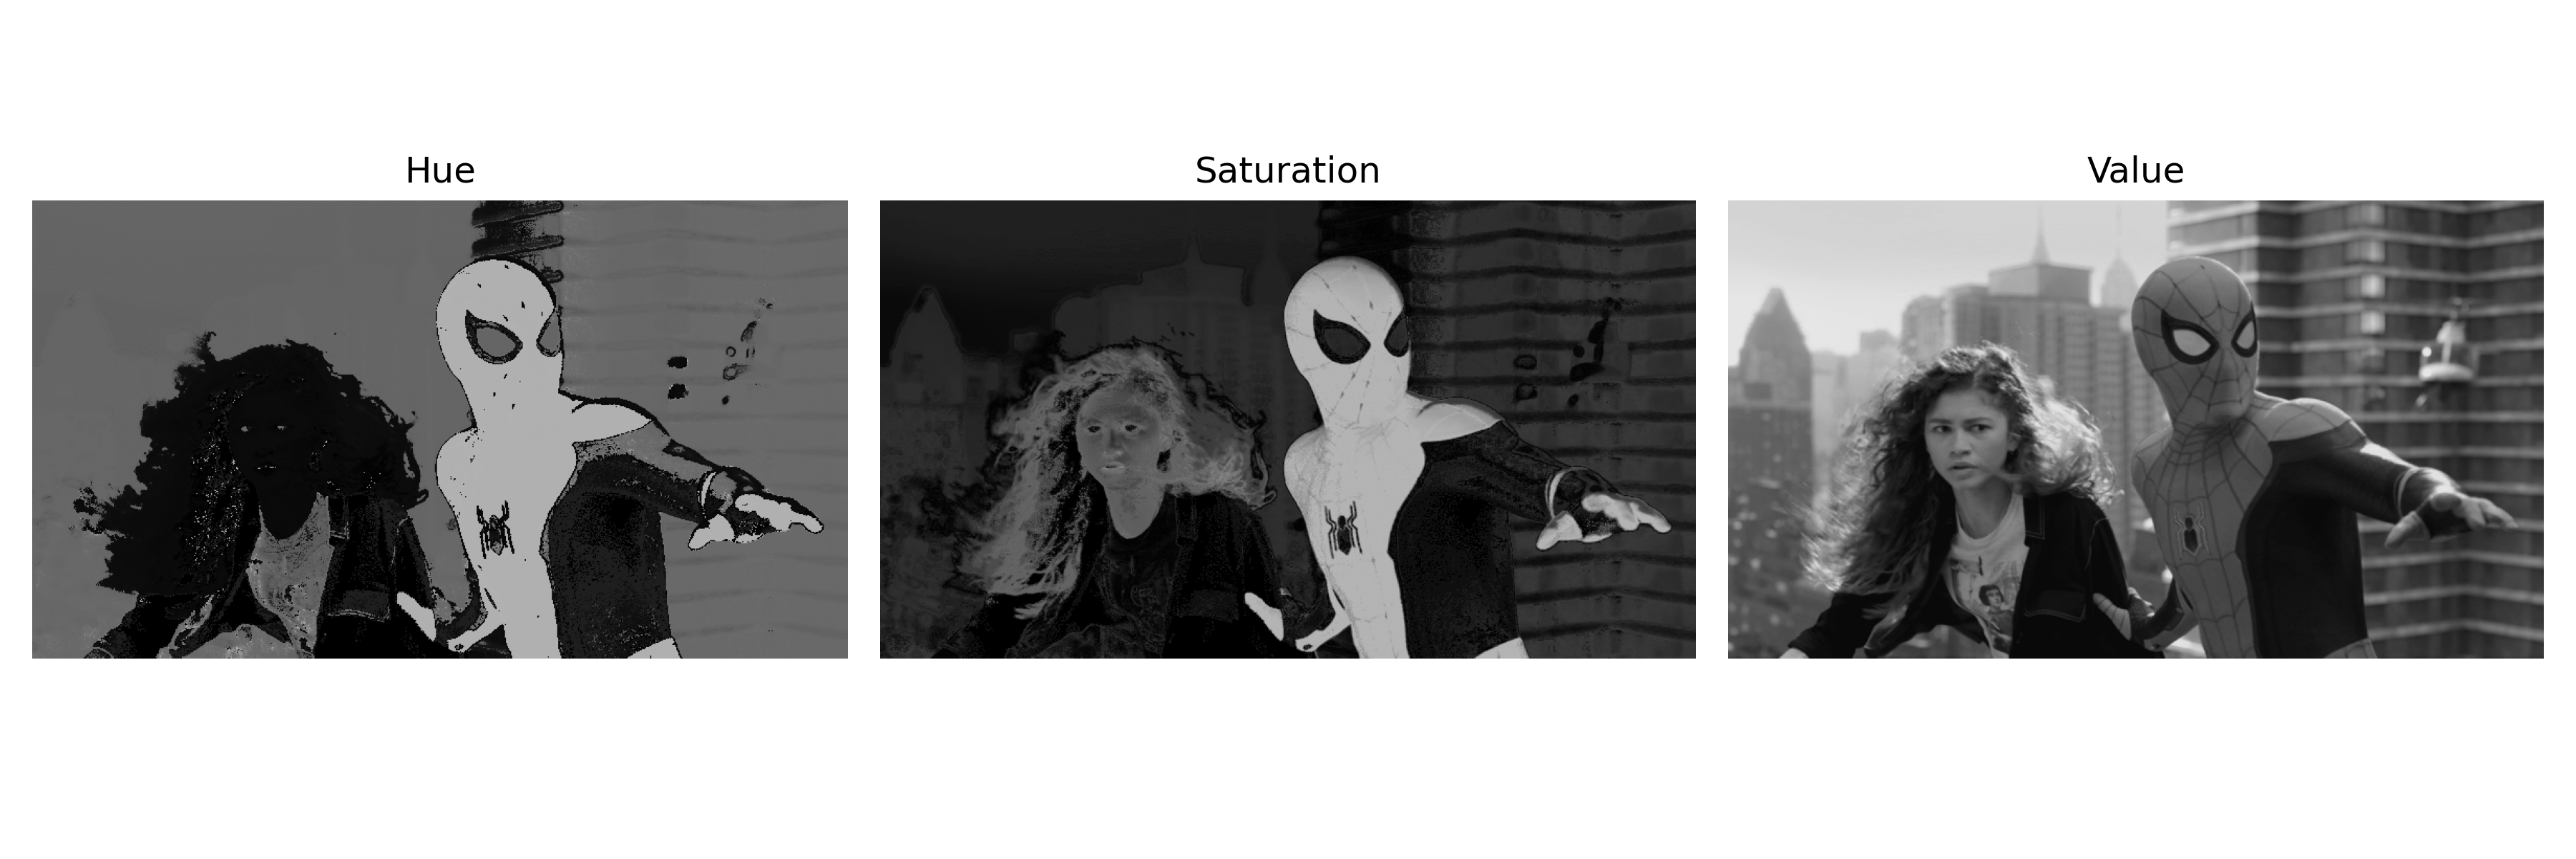
\includegraphics[width=\textwidth]{task4/hsv_planes.png}
    \caption{HSV channel separation}
\end{figure}
\begin{figure}[H]
    \centering
        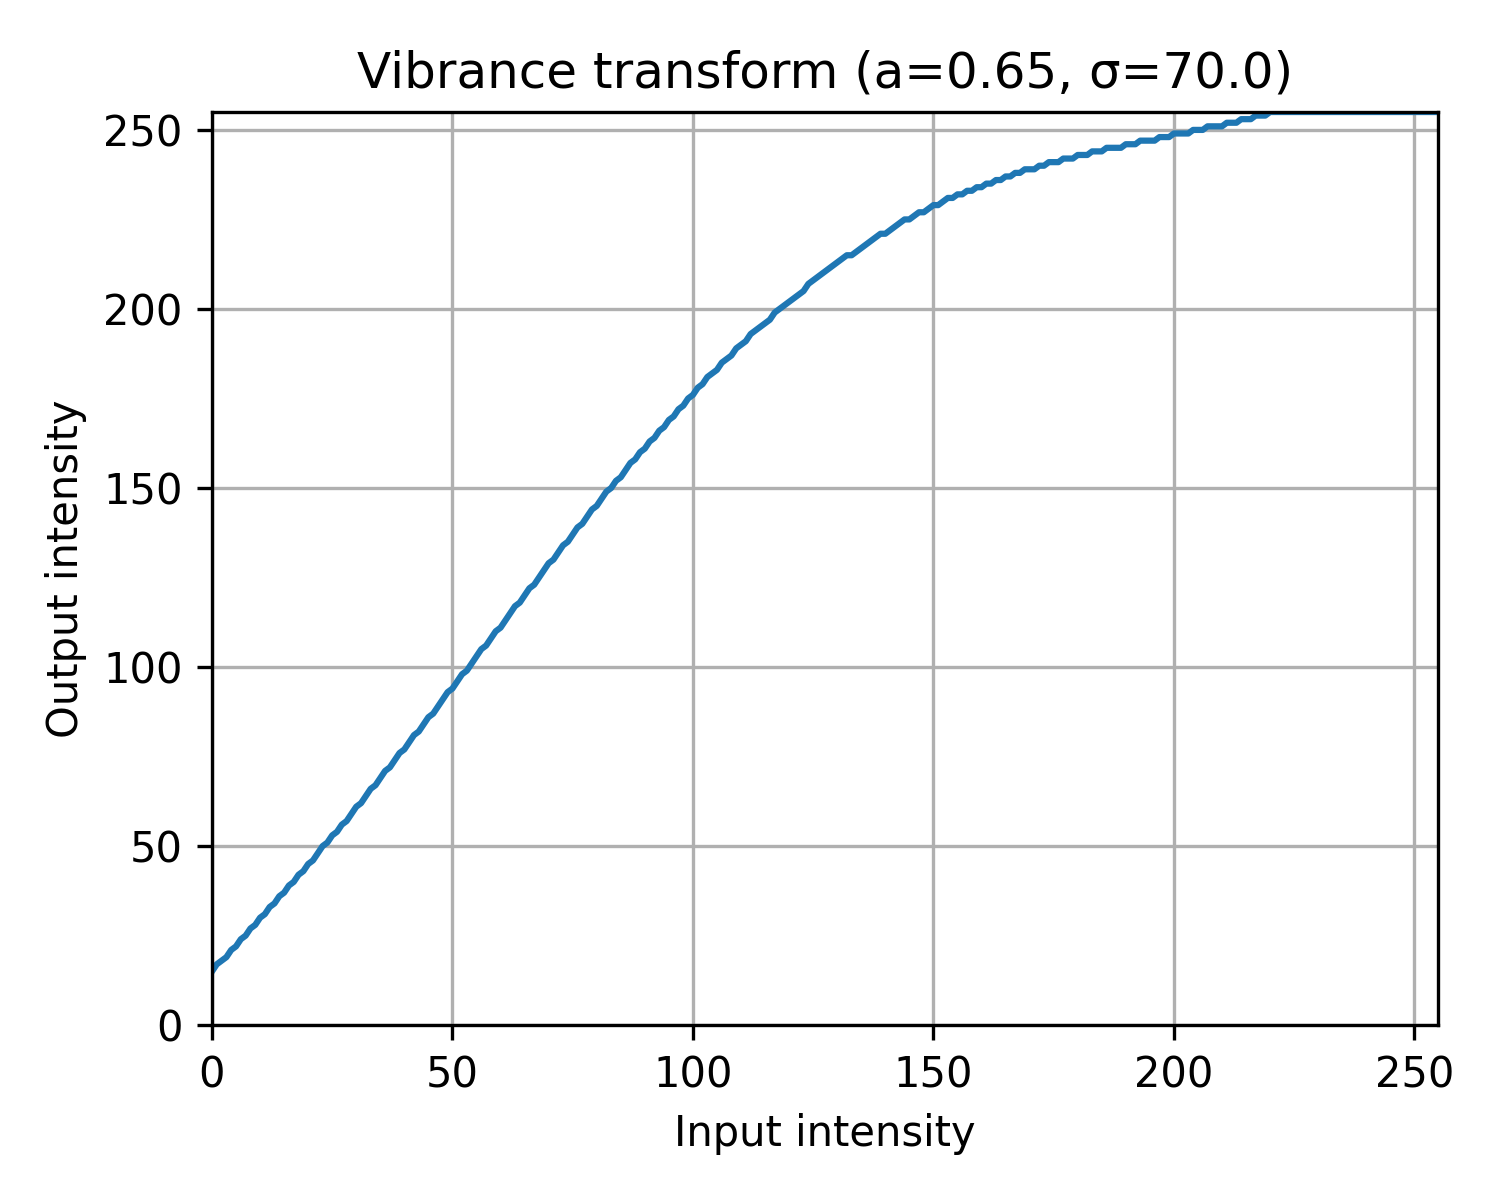
\includegraphics[width=0.4\textwidth]{task4/transform_curve.png}
        \caption{Vibrance transformation}
\end{figure}

\begin{figure}[H]
    \centering
    \begin{subfigure}{0.48\textwidth}
        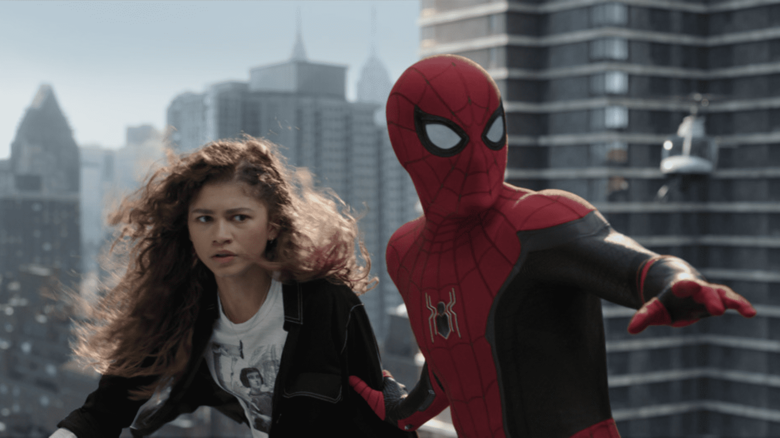
\includegraphics[width=\textwidth]{task4/original.png}
        \caption{Original image}
    \end{subfigure}
    \begin{subfigure}{0.48\textwidth}
        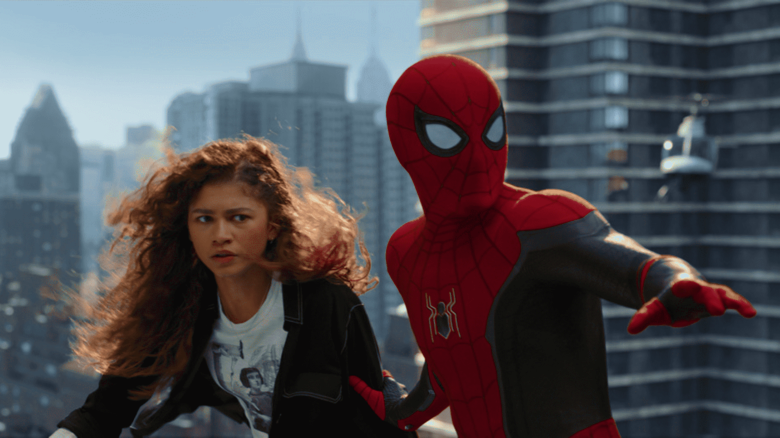
\includegraphics[width=\textwidth]{task4/enhanced.png}
        \caption{Enhanced result (a = 0.65)}
    \end{subfigure}
    \caption{Vibrance enhancement results}
\end{figure}

\textbf{Interpretation:} The transformation selectively enhances colorful regions while preserving grayscale areas, effectively increasing image vibrance.

\section{Question 5}
Custom histogram equalization was implemented to spread the intensity distribution uniformly across the full dynamic range.

\begin{lstlisting}[caption=Custom histogram equalization function]
def my_hist_equalization(img):
    L = 256
    M, N = img.shape
    hist = cv.calcHist([img], [0], None, [L], [0, L])
    cdf = hist.cumsum()

    t = np.array([(L - 1) / (M * N) * cdf[K] for K in range(L)]).astype("uint8")
    return t[img]

\end{lstlisting}

\begin{figure}[H]
    \centering
    \begin{subfigure}{0.48\textwidth}
        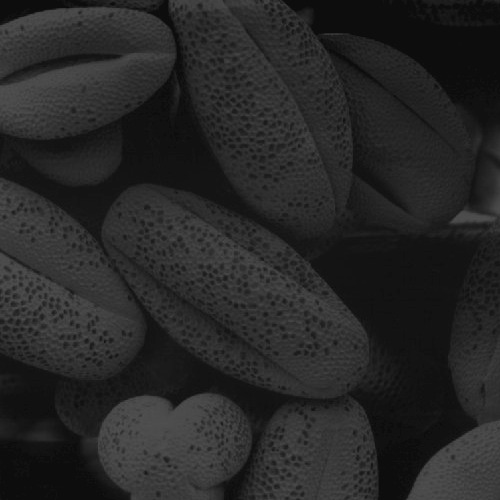
\includegraphics[width=\textwidth]{task5/shells.jpg}
        \caption{Original image}
    \end{subfigure}
    \hfill
    \begin{subfigure}{0.48\textwidth}
        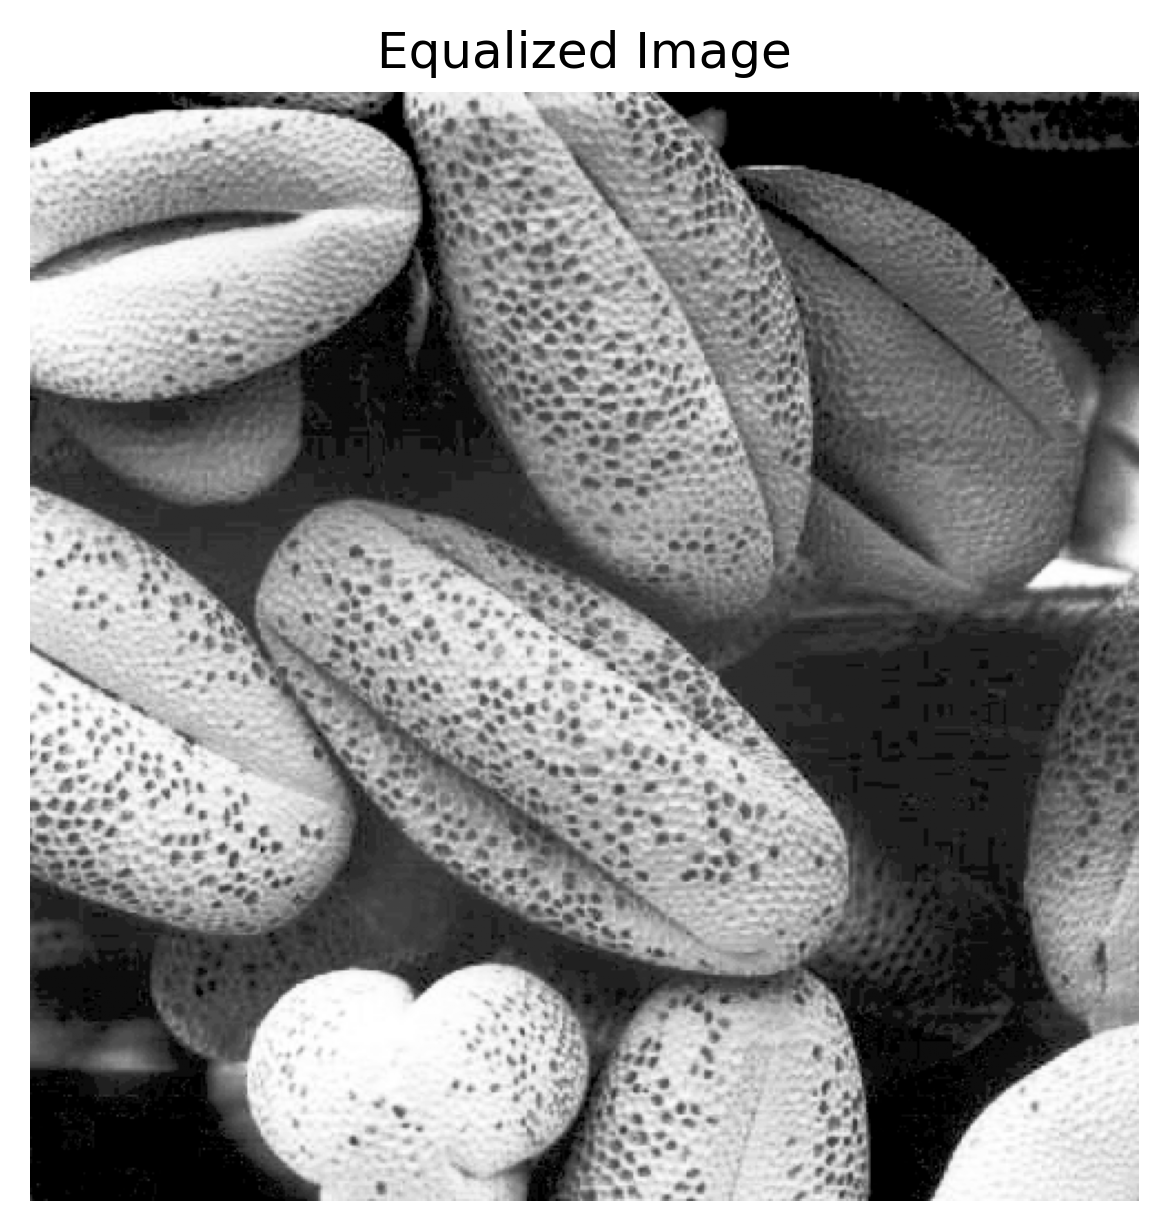
\includegraphics[width=\textwidth]{task5/2_equalized_image.png}
        \caption{Equalized image}
    \end{subfigure}
    \caption{Histogram equalization results}
\end{figure}

\begin{figure}[H]
    \centering
    \begin{subfigure}{0.48\textwidth}
        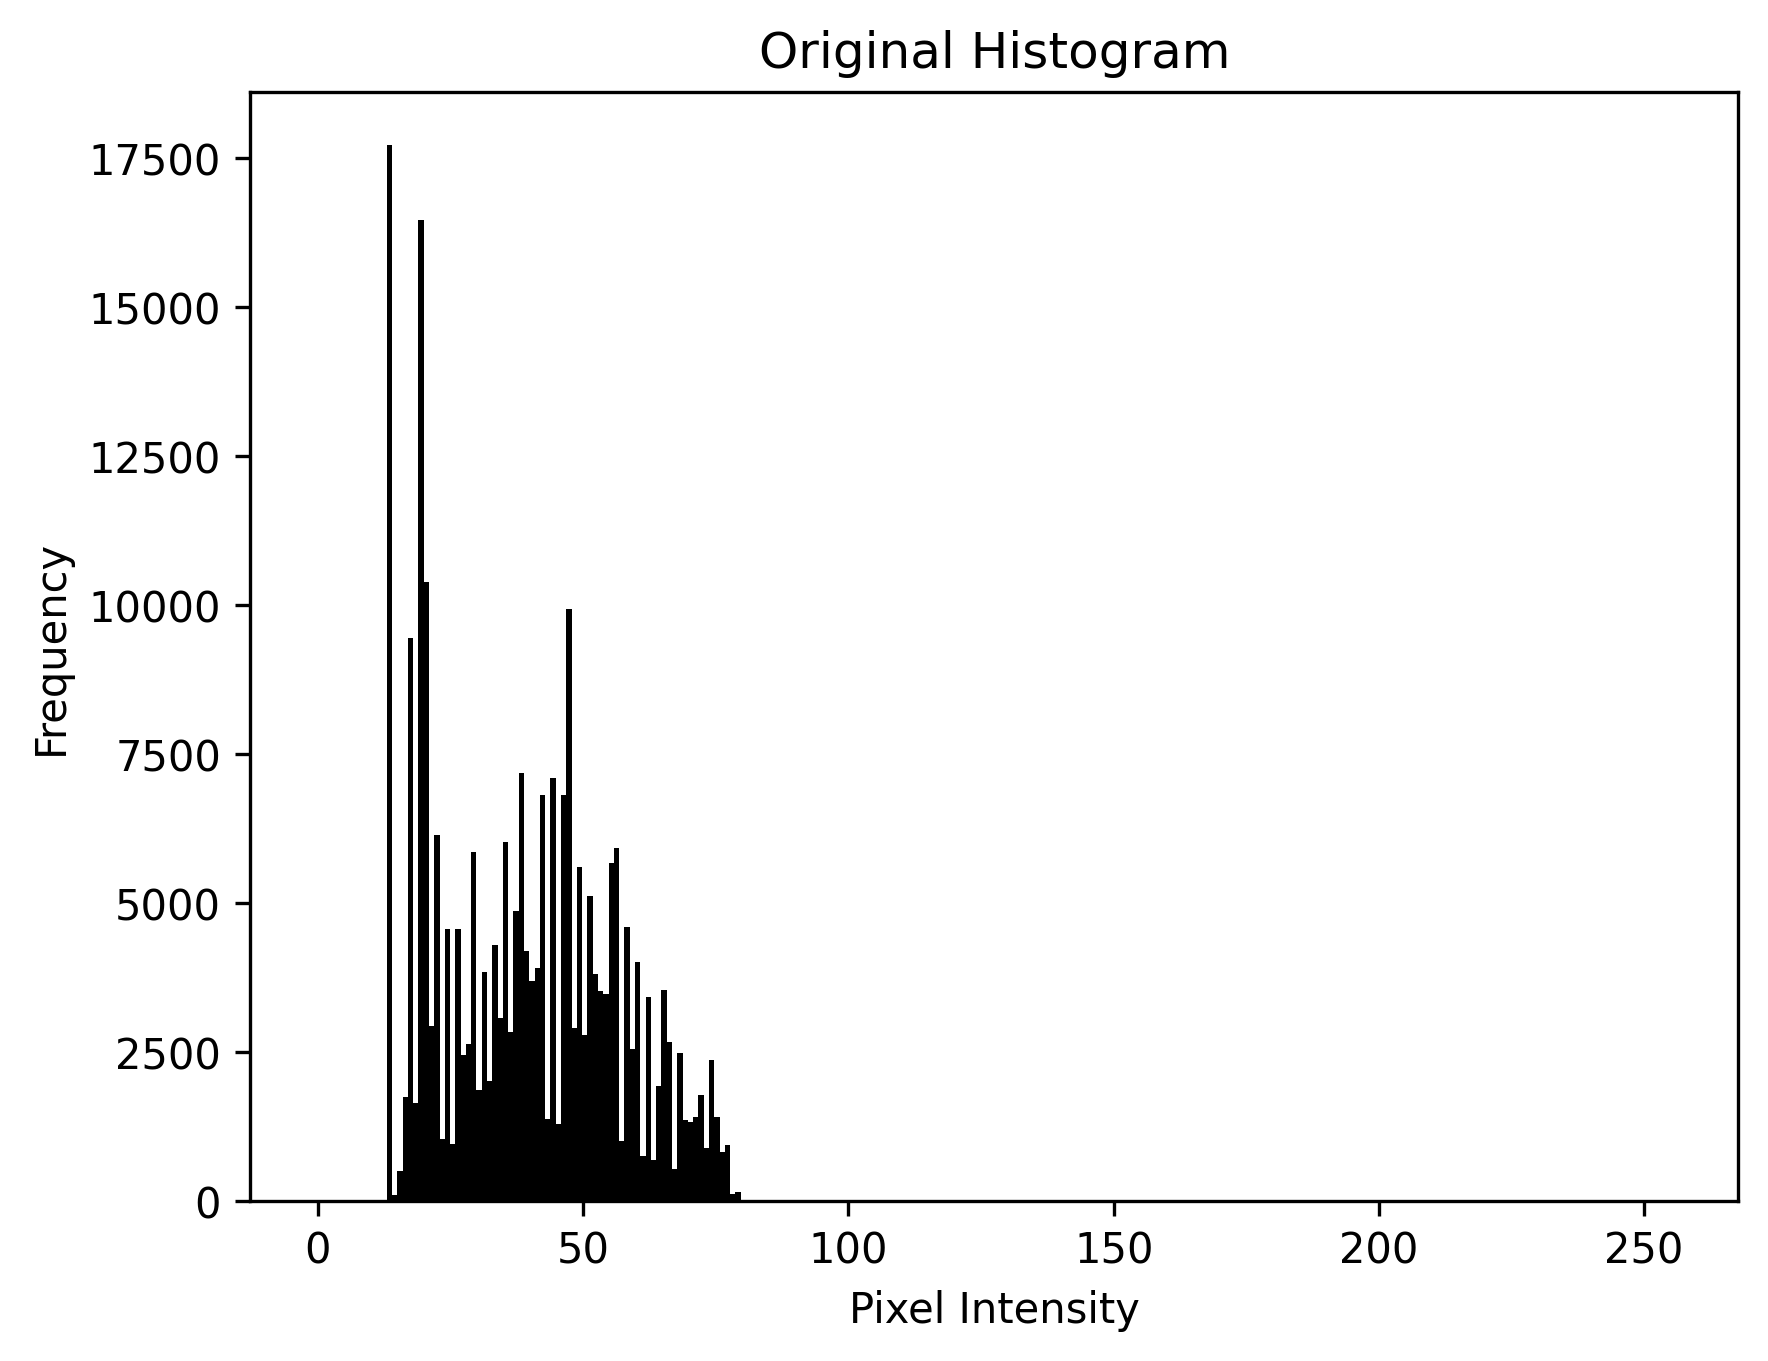
\includegraphics[width=\textwidth]{task5/3_original_histogram.png}
        \caption{Original histogram}
    \end{subfigure}
    \hfill
    \begin{subfigure}{0.48\textwidth}
        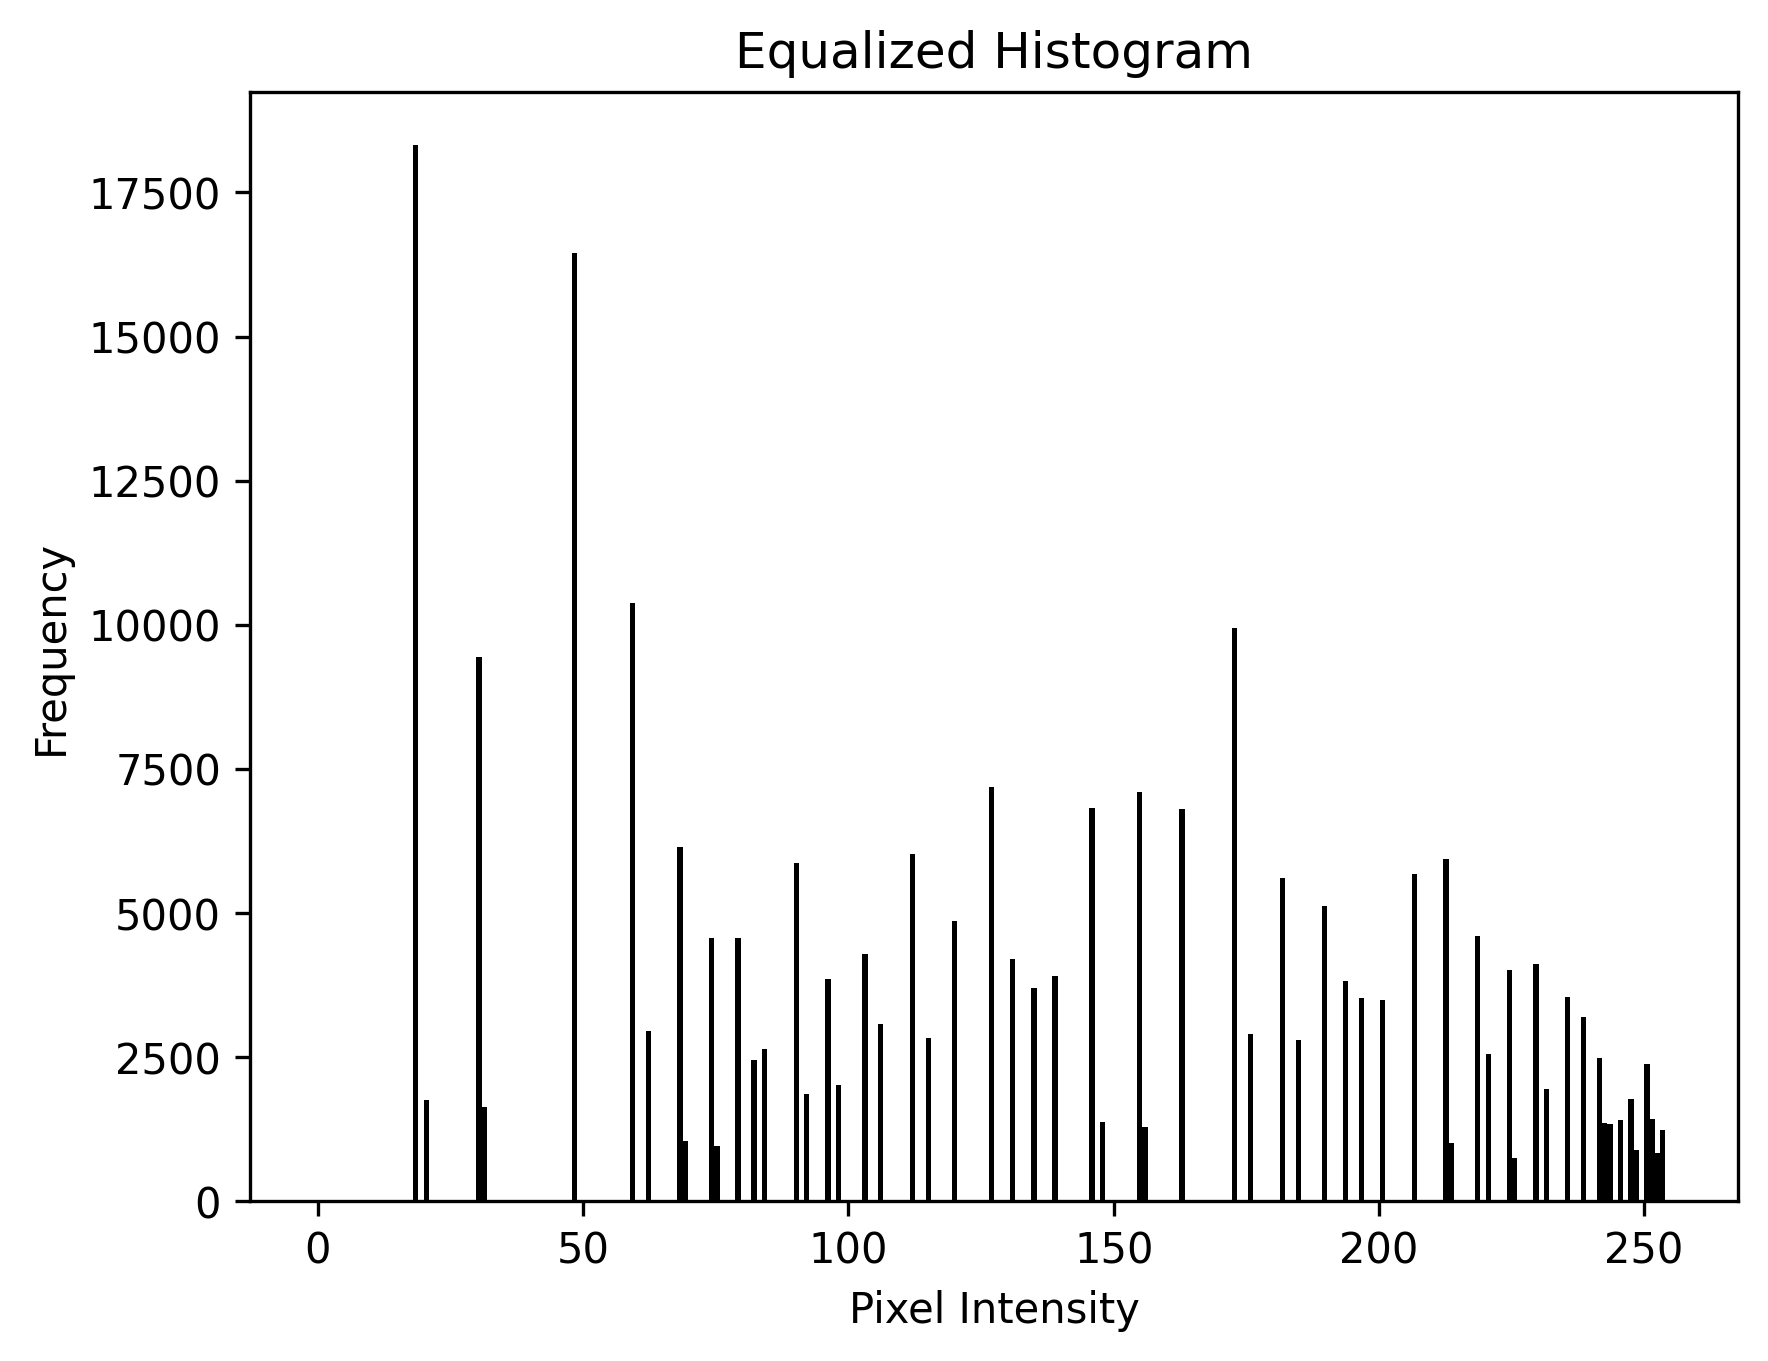
\includegraphics[width=\textwidth]{task5/4_equalized_histogram.png}
        \caption{Equalized histogram}
    \end{subfigure}
    \caption{Histogram comparison}
\end{figure}


\textbf{Interpretation:} The equalization process spreads the histogram more uniformly, improving overall contrast and detail visibility.

\section{Question 6}
Selective histogram equalization was applied only to the foreground region using mask-based processing. The saturation plane was used to create a mask that isolates the foreground.

\begin{lstlisting}[caption=Foreground histogram equalization]
# Convert to HSV and split channels
img_hsv = cv.cvtColor(img_bgr, cv.COLOR_BGR2HSV)
h, s, v = cv.split(img_hsv)

# Create mask using Saturation channel
_, mask = cv.threshold(s, 12, 255, cv.THRESH_BINARY)

# Extract foreground
foreground = cv.bitwise_and(img_bgr, img_bgr, mask=mask)

foreground_hsv = cv.cvtColor(foreground, cv.COLOR_BGR2HSV)
H_fg, S_fg, V_fg = cv.split(foreground_hsv)

hist = cv.calcHist([V_fg], [0], mask, [256], [0, 256])
x_positions = np.arange(len(hist))

cdf = hist.cumsum()

# Equalize only the foreground
v_eq = my_hist_equalization(V_fg, cdf)
hist_eq = cv.calcHist([v_eq], [0], mask, [256], [0, 256])
x_positions_eq = np.arange(len(hist_eq))

# Merge back channels
hsv_eq = cv.merge([H_fg, S_fg, v_eq])
modified_fg = cv.cvtColor(hsv_eq, cv.COLOR_HSV2BGR)

background = cv.bitwise_and(img_bgr, img_bgr, mask=cv.bitwise_not(mask))
final_img_bgr = cv.add(cv.cvtColor(background, cv.COLOR_BGR2RGB), modified_fg)
\end{lstlisting}


\begin{figure}
    \centering
        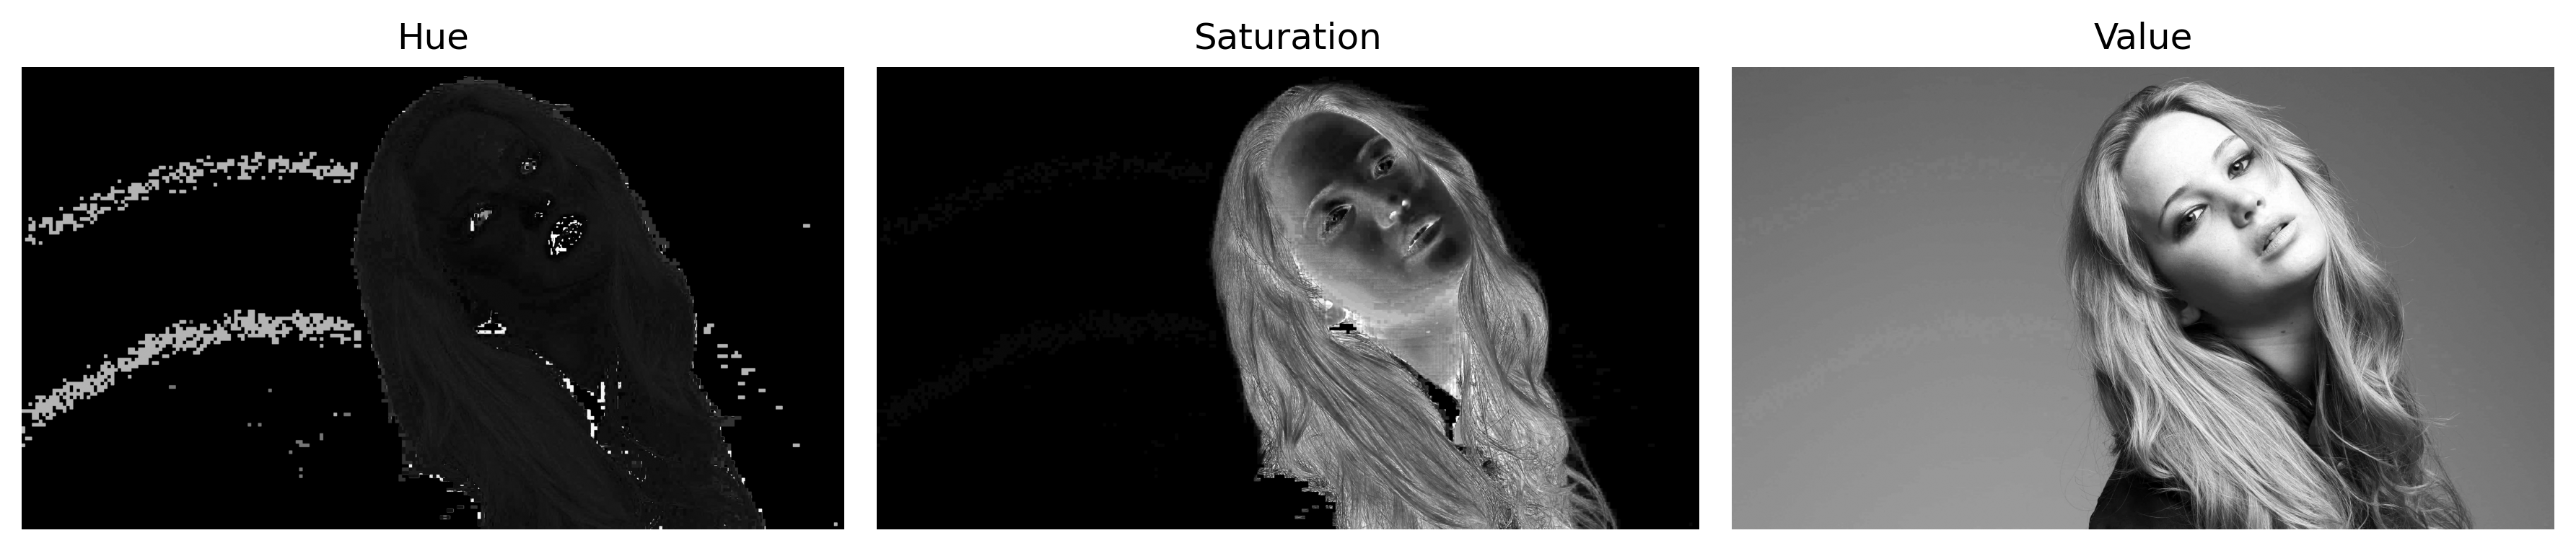
\includegraphics[width=\textwidth]{task6/1_hsv_planes.png}
        \caption{HSV planes}
\end{figure}

\begin{figure}[H]
    \centering
    \begin{subfigure}{0.24\textwidth}
        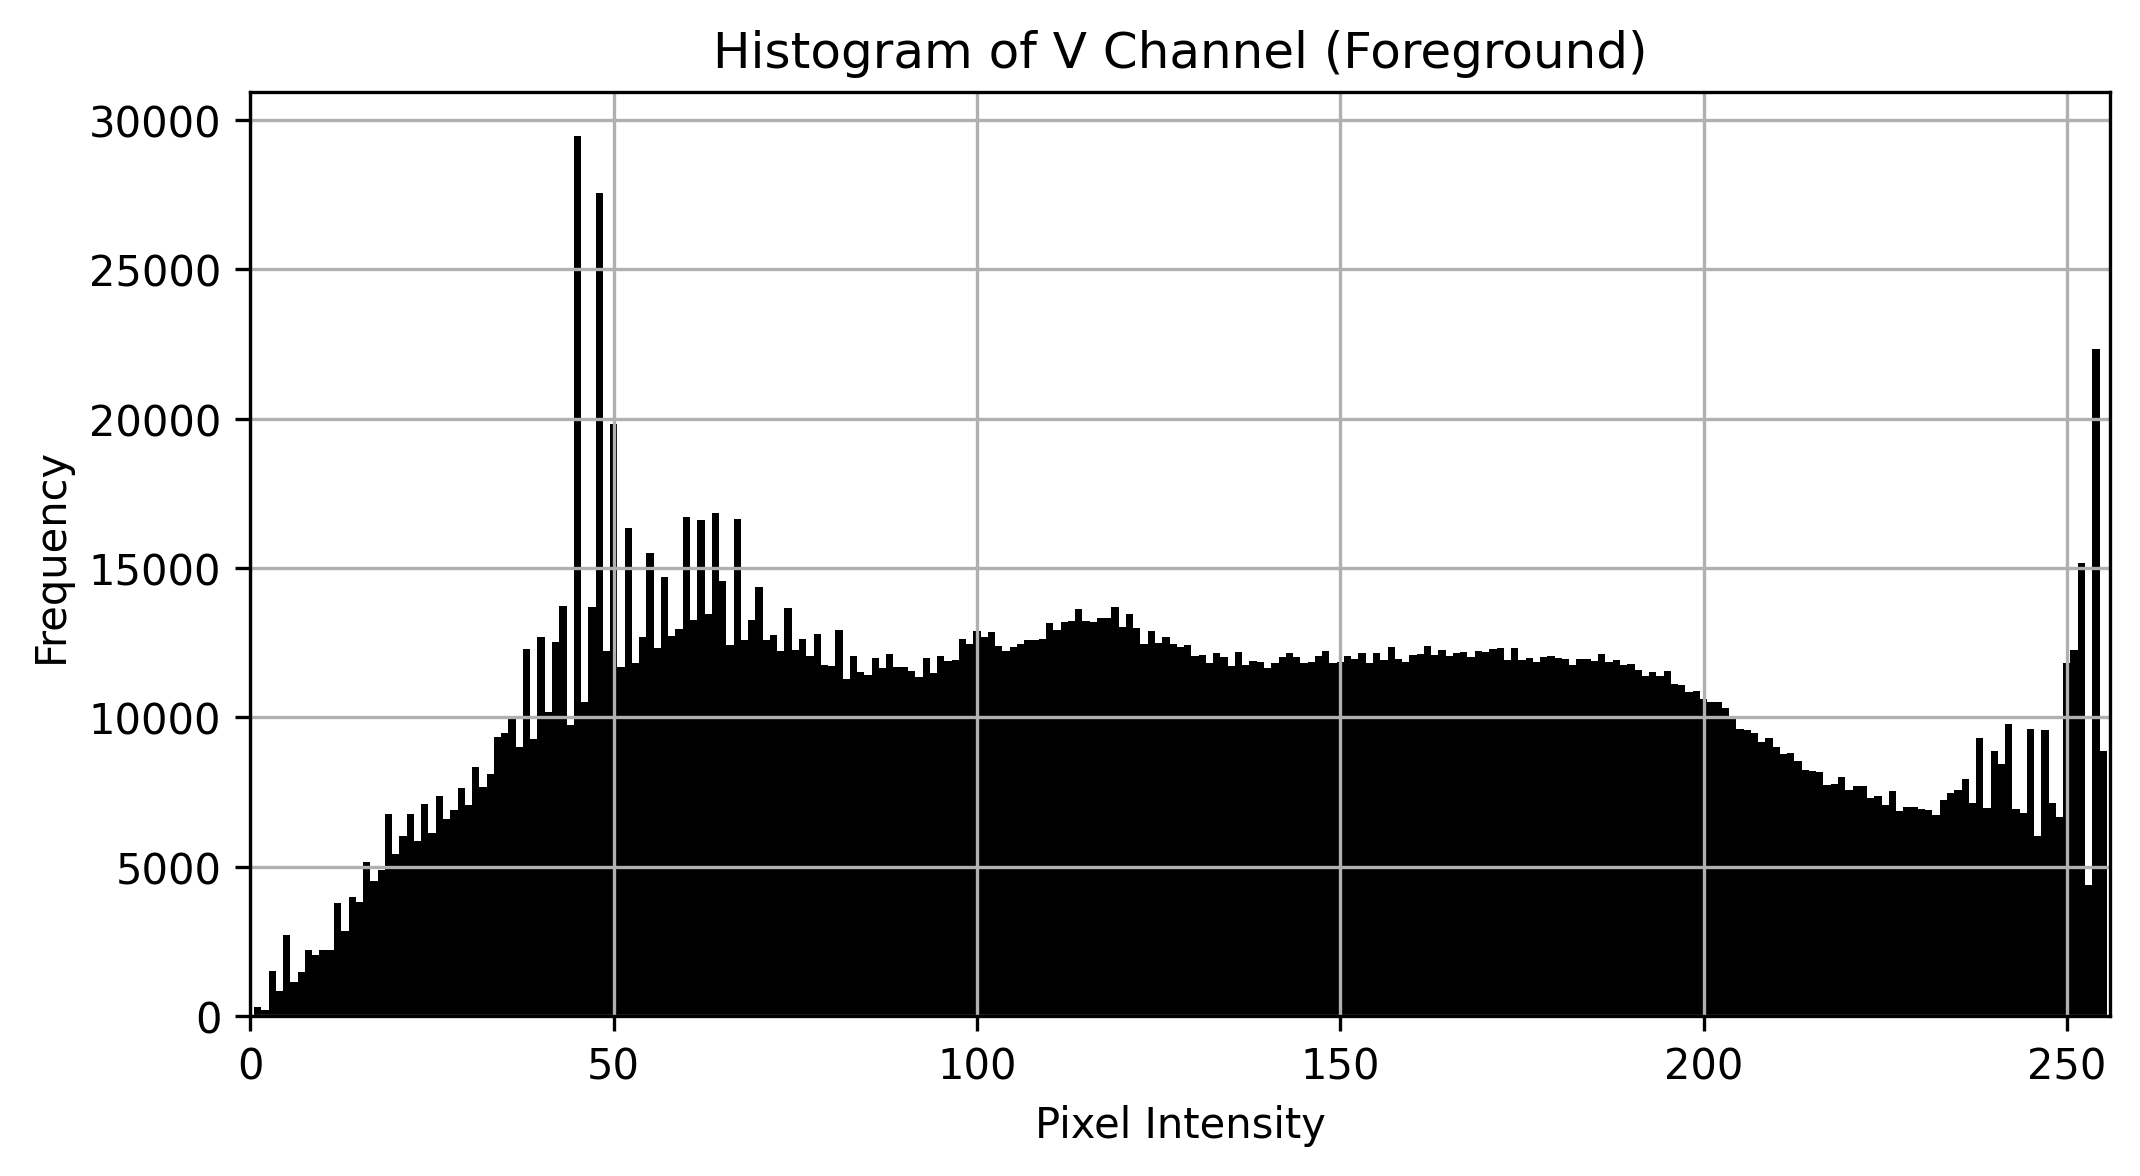
\includegraphics[width=\textwidth]{task6/6_histogram.png}
        \caption{original histogram }
    \end{subfigure}
    \begin{subfigure}{0.24\textwidth}
        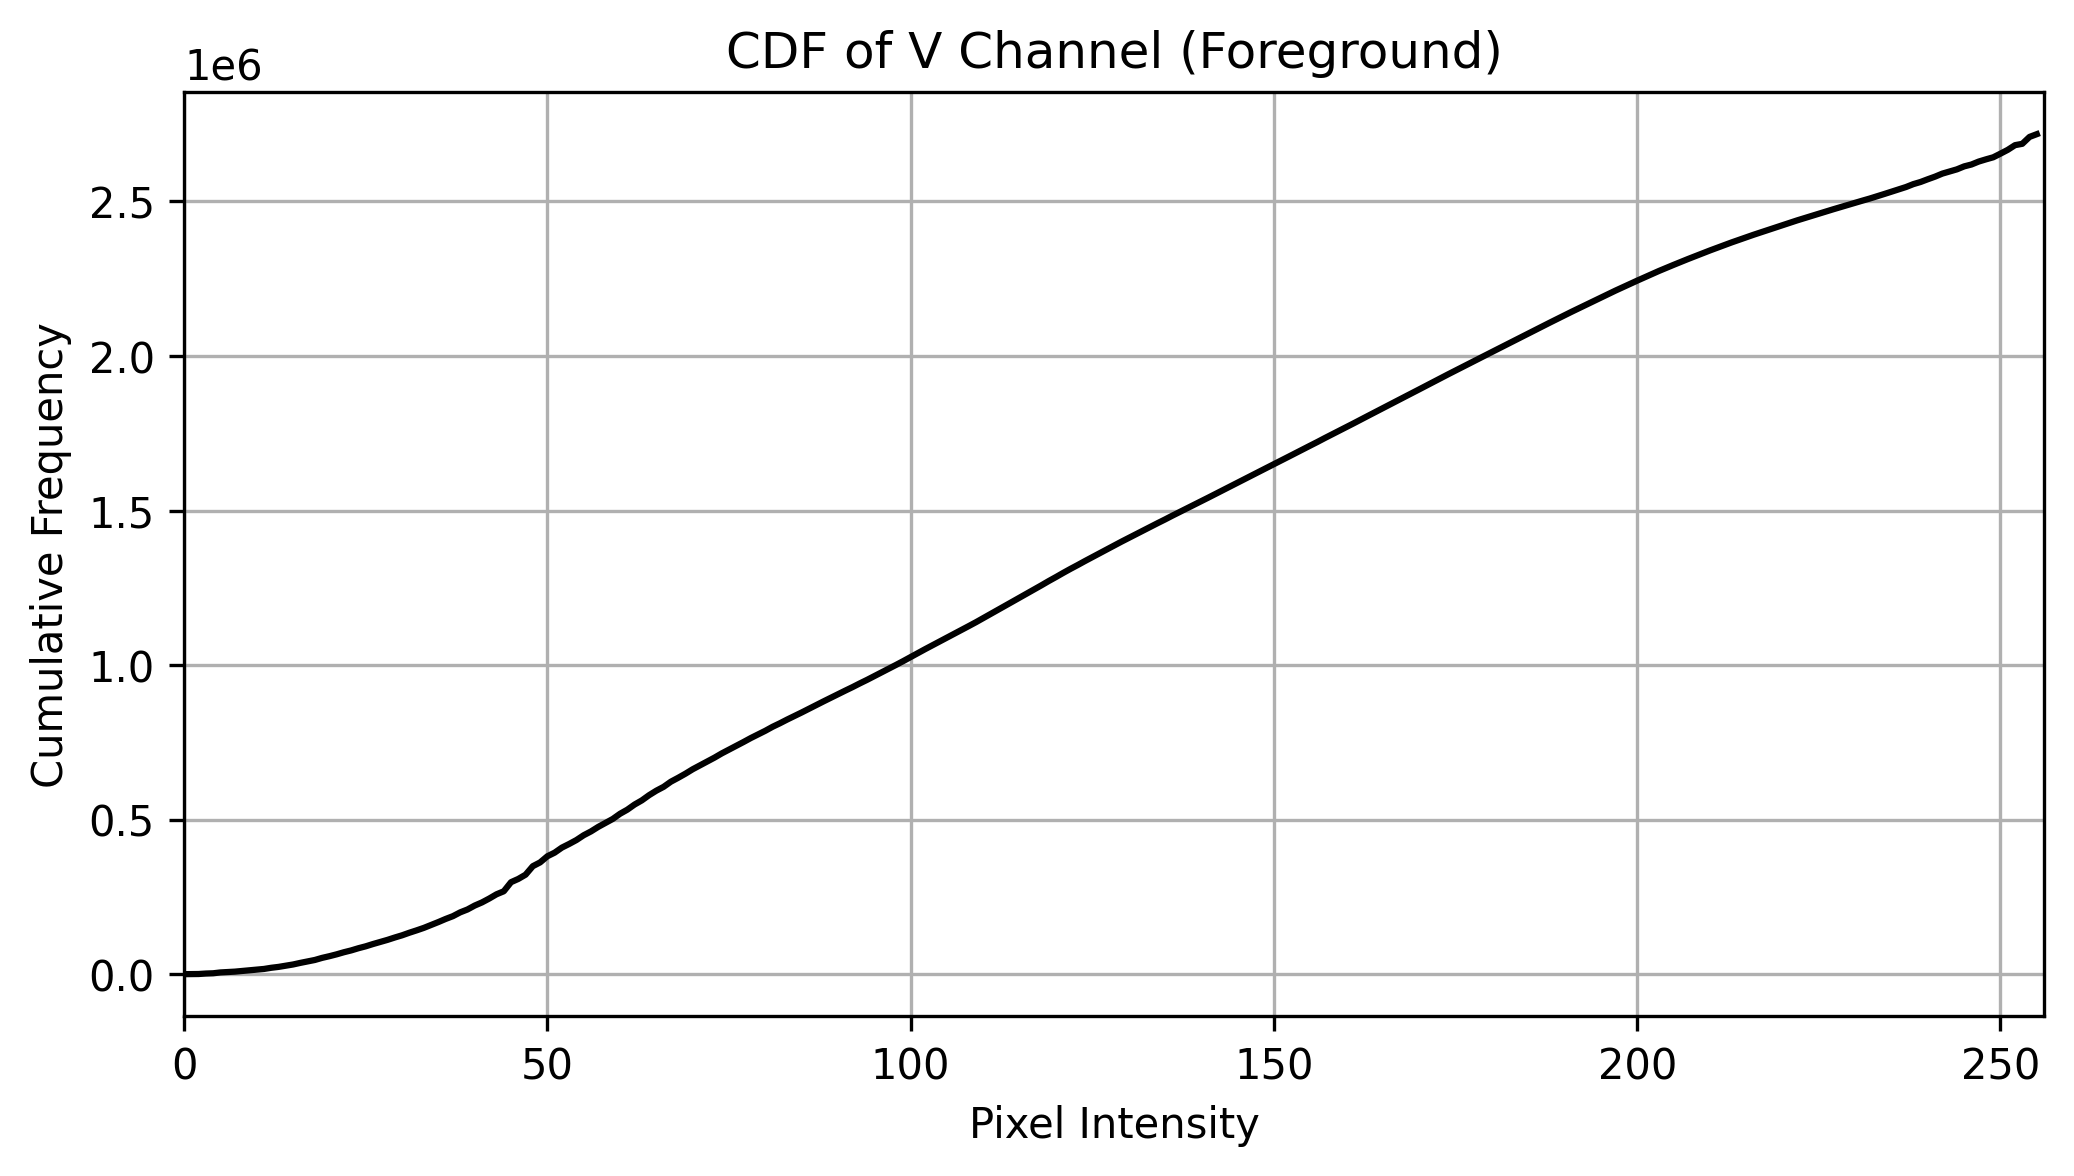
\includegraphics[width=\textwidth]{task6/7_cdf.png}
        \caption{Original CDF}
    \end{subfigure}
    \begin{subfigure}{0.24\textwidth}
        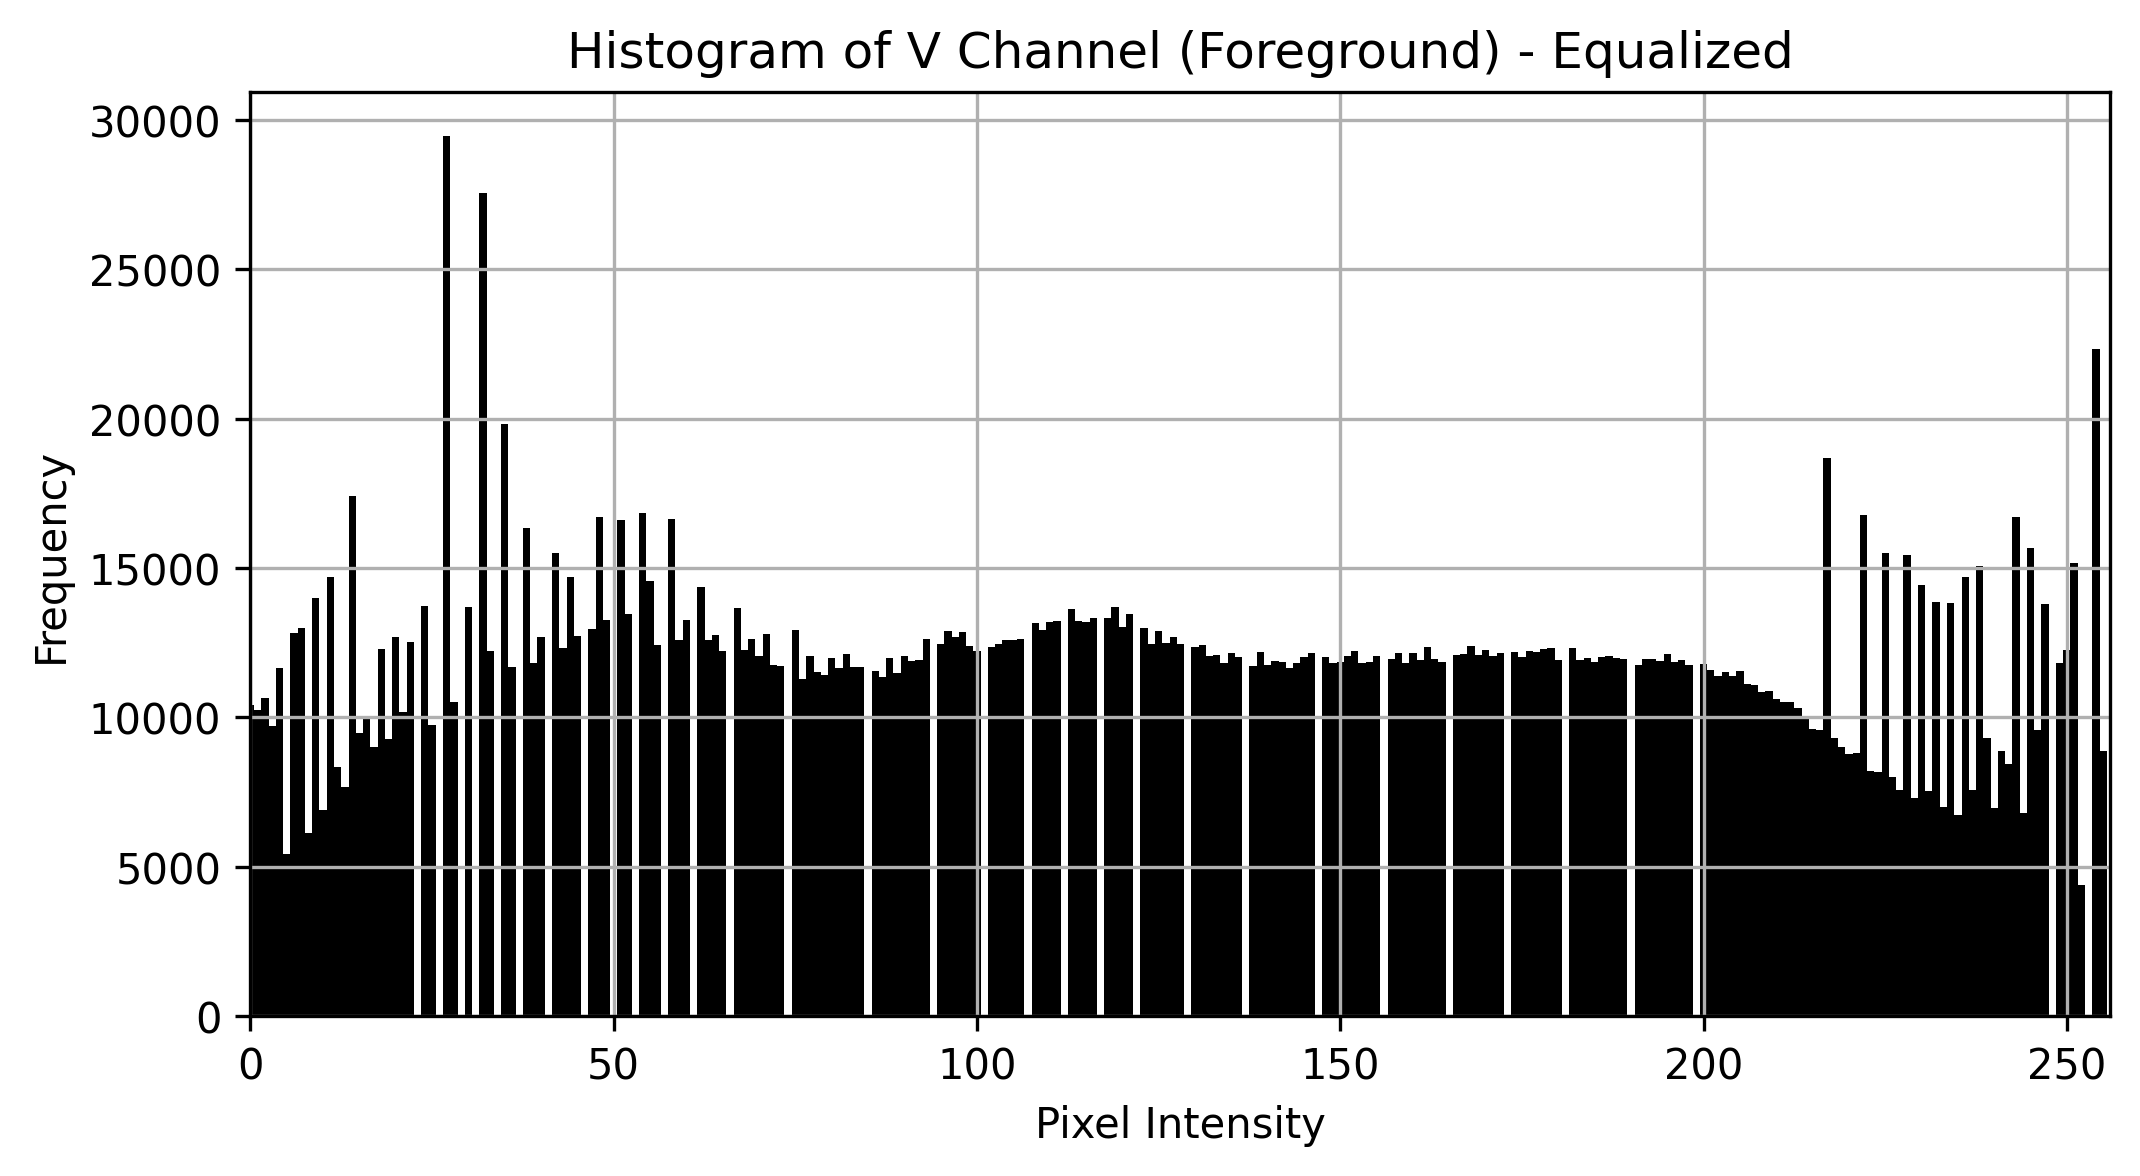
\includegraphics[width=\textwidth]{task6/8_histogram_eq.png}
        \caption{equalized histogram}
    \end{subfigure}
    \caption{Foreground histogram equalization process}
\end{figure}

\begin{figure}[H]
    \centering
    \begin{subfigure}{0.24\textwidth}
        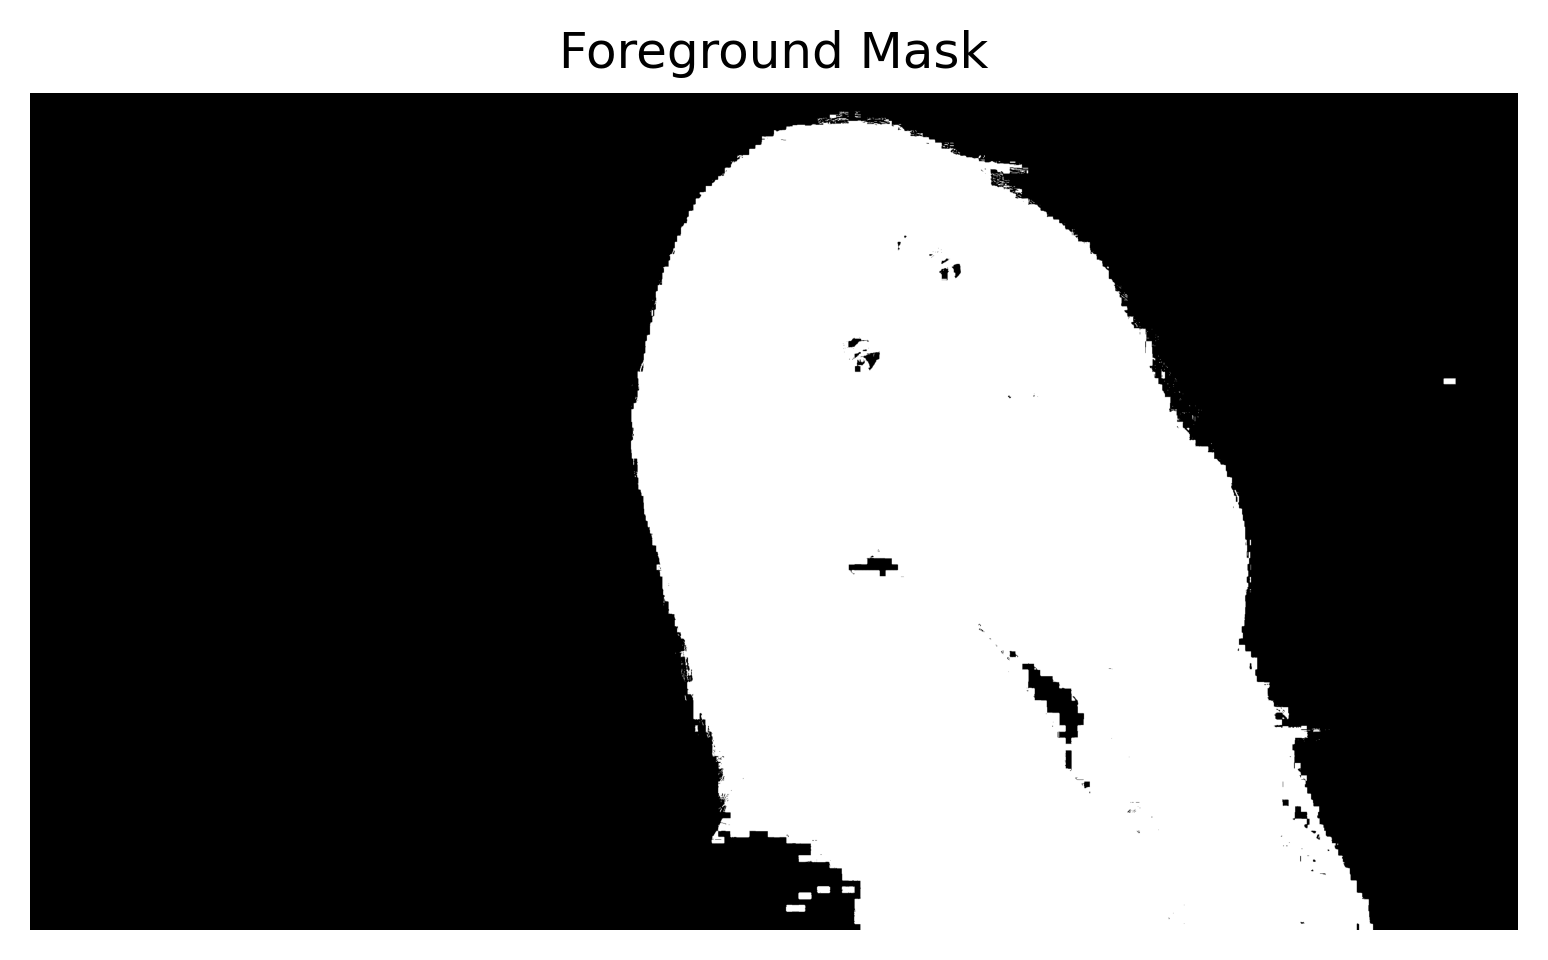
\includegraphics[width=\textwidth]{task6/2_mask.png}
        \caption{Foreground mask}
    \end{subfigure}
    \begin{subfigure}{0.24\textwidth}
        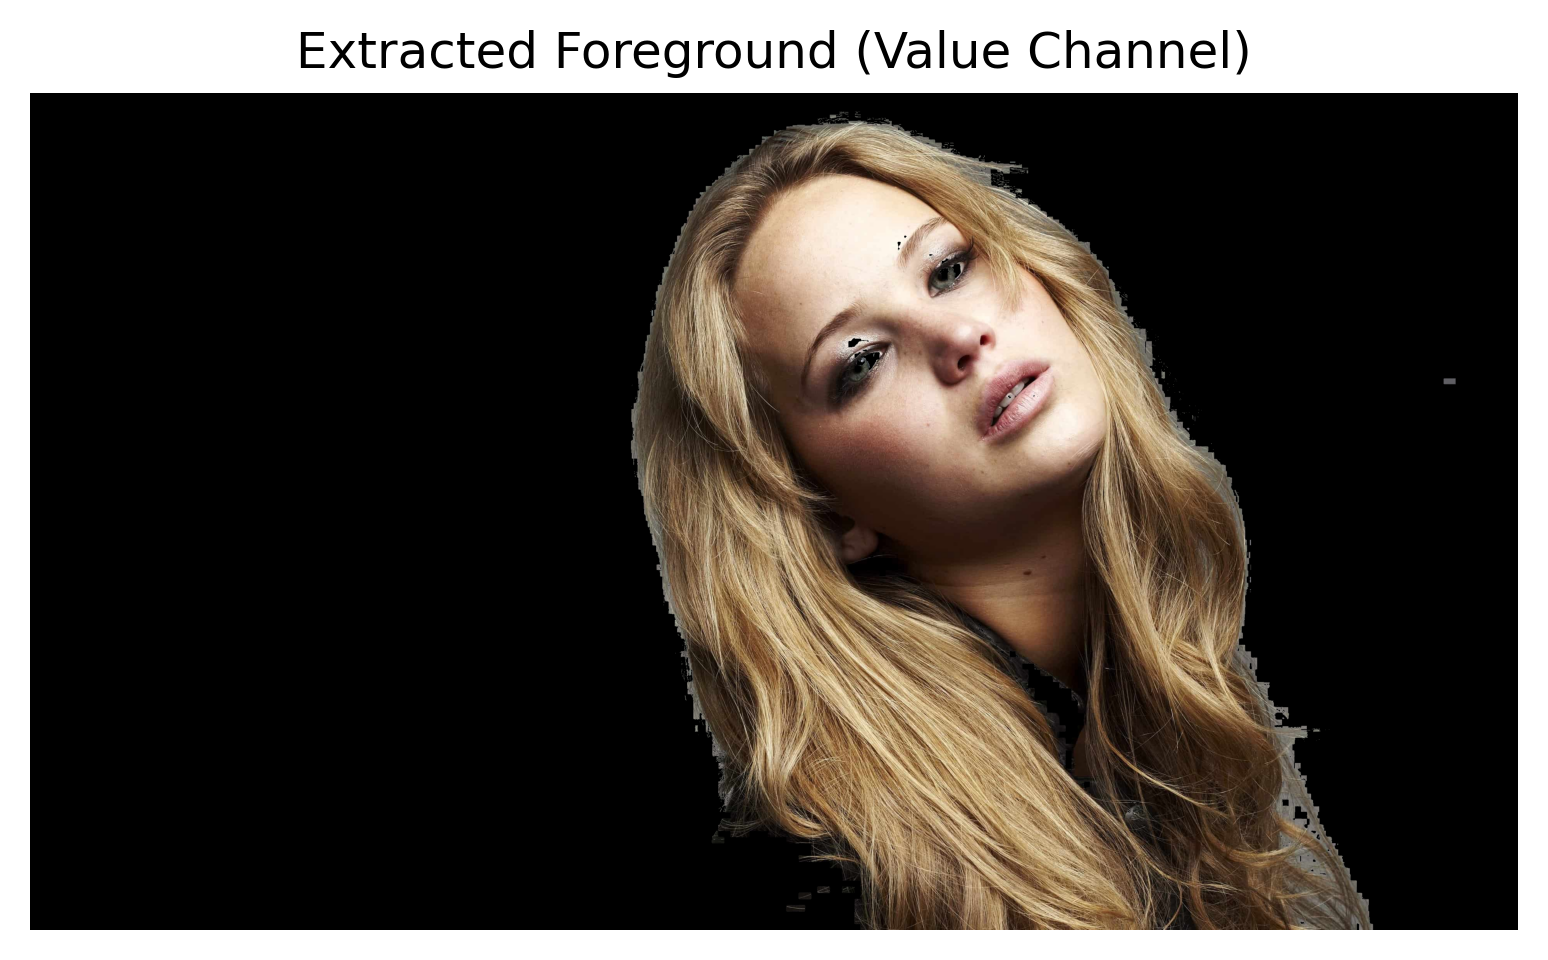
\includegraphics[width=\textwidth]{task6/3_foreground.png}
        \caption{Extracted foreground}
    \end{subfigure}
    \begin{subfigure}{0.24\textwidth}
        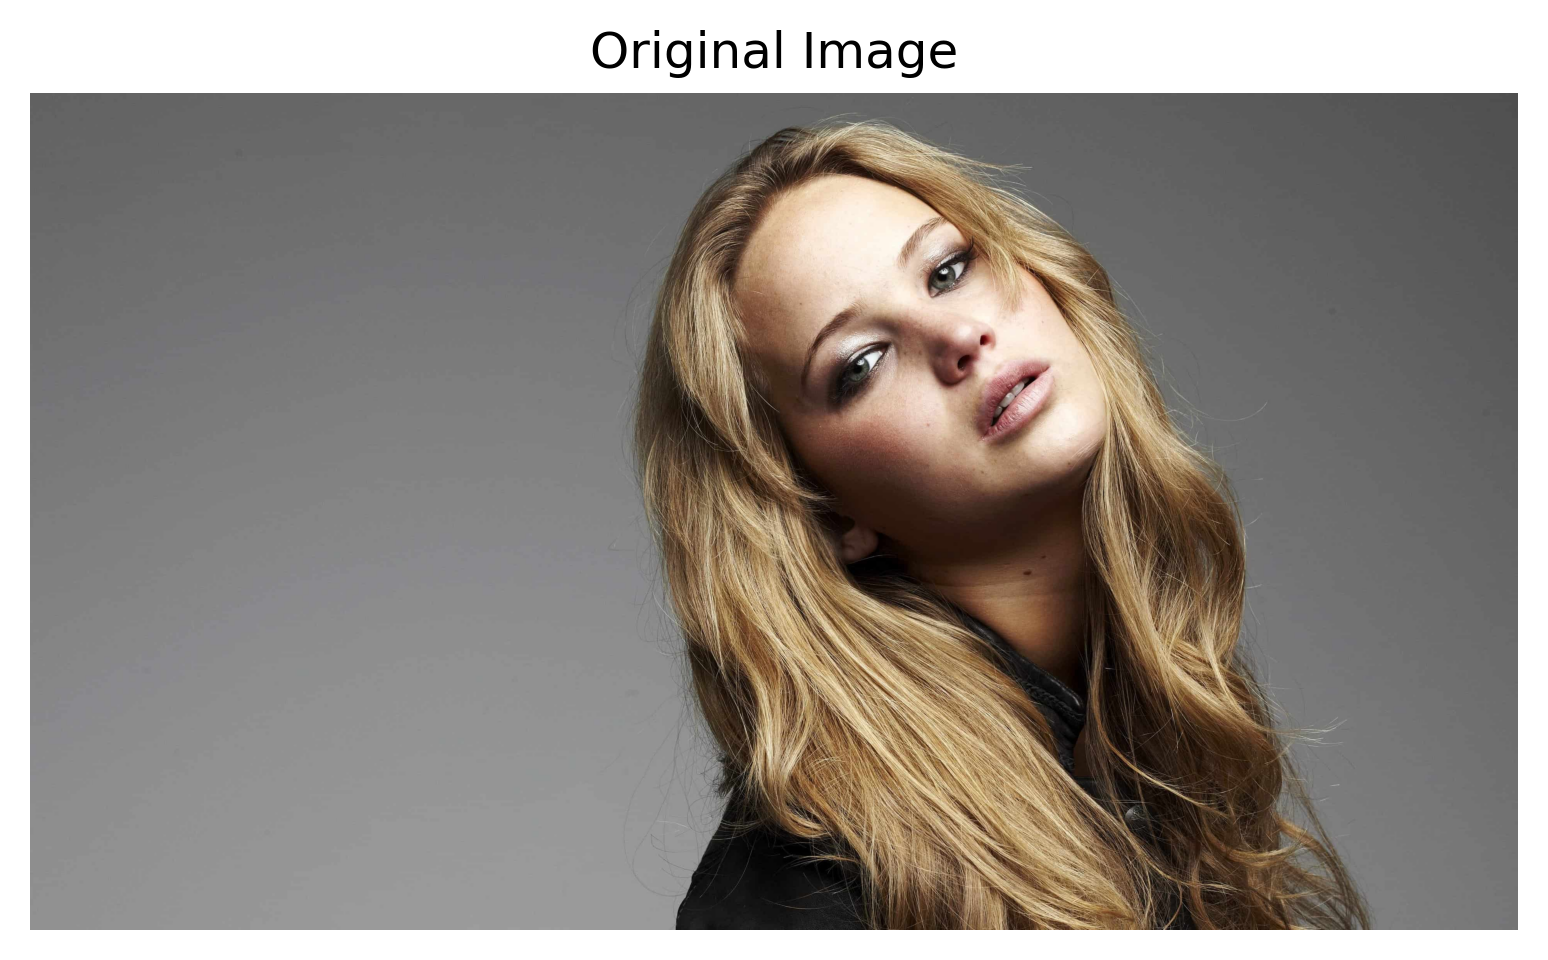
\includegraphics[width=\textwidth]{task6/4_original.png}
        \caption{Original image}
    \end{subfigure}
    \begin{subfigure}{0.24\textwidth}
        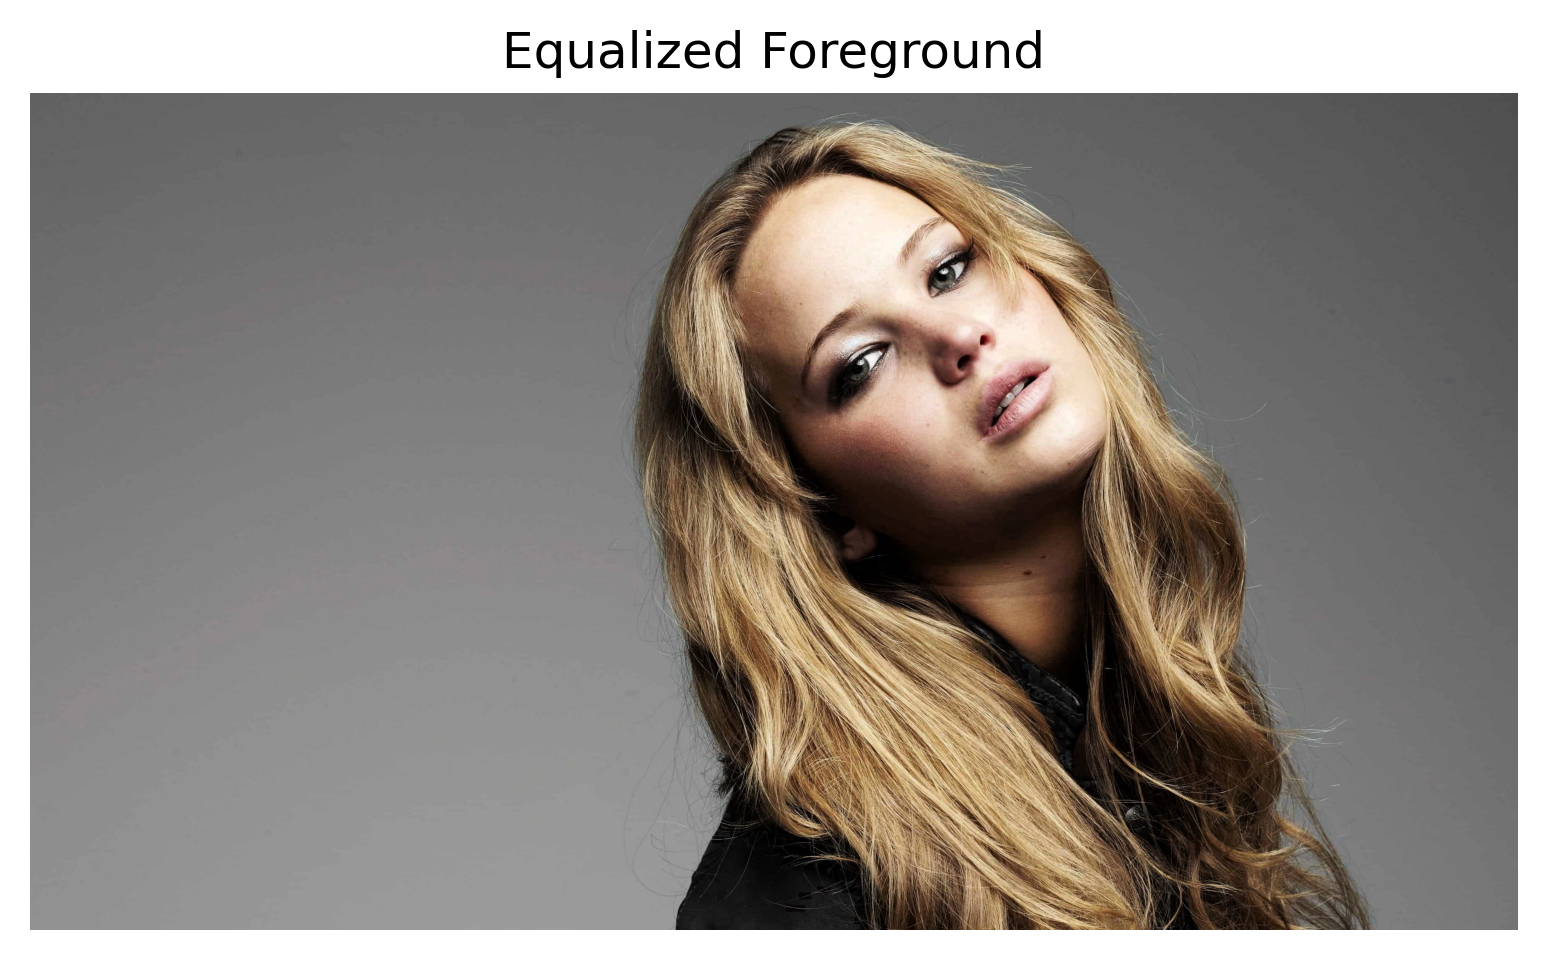
\includegraphics[width=\textwidth]{task6/5_result.png}
        \caption{Final result}
    \end{subfigure}
    \caption{Foreground histogram equalization process}
\end{figure}

\textbf{Interpretation:} Selective equalization enhances foreground details while preserving the background, resulting in improved subject contrast.

\section{Question 7}
Sobel filtering was implemented using three different approaches: OpenCV's filter2D, custom 2D convolution, and separable convolution.


\begin{figure}[H]
    \centering
    \begin{subfigure}{0.48\textwidth}
        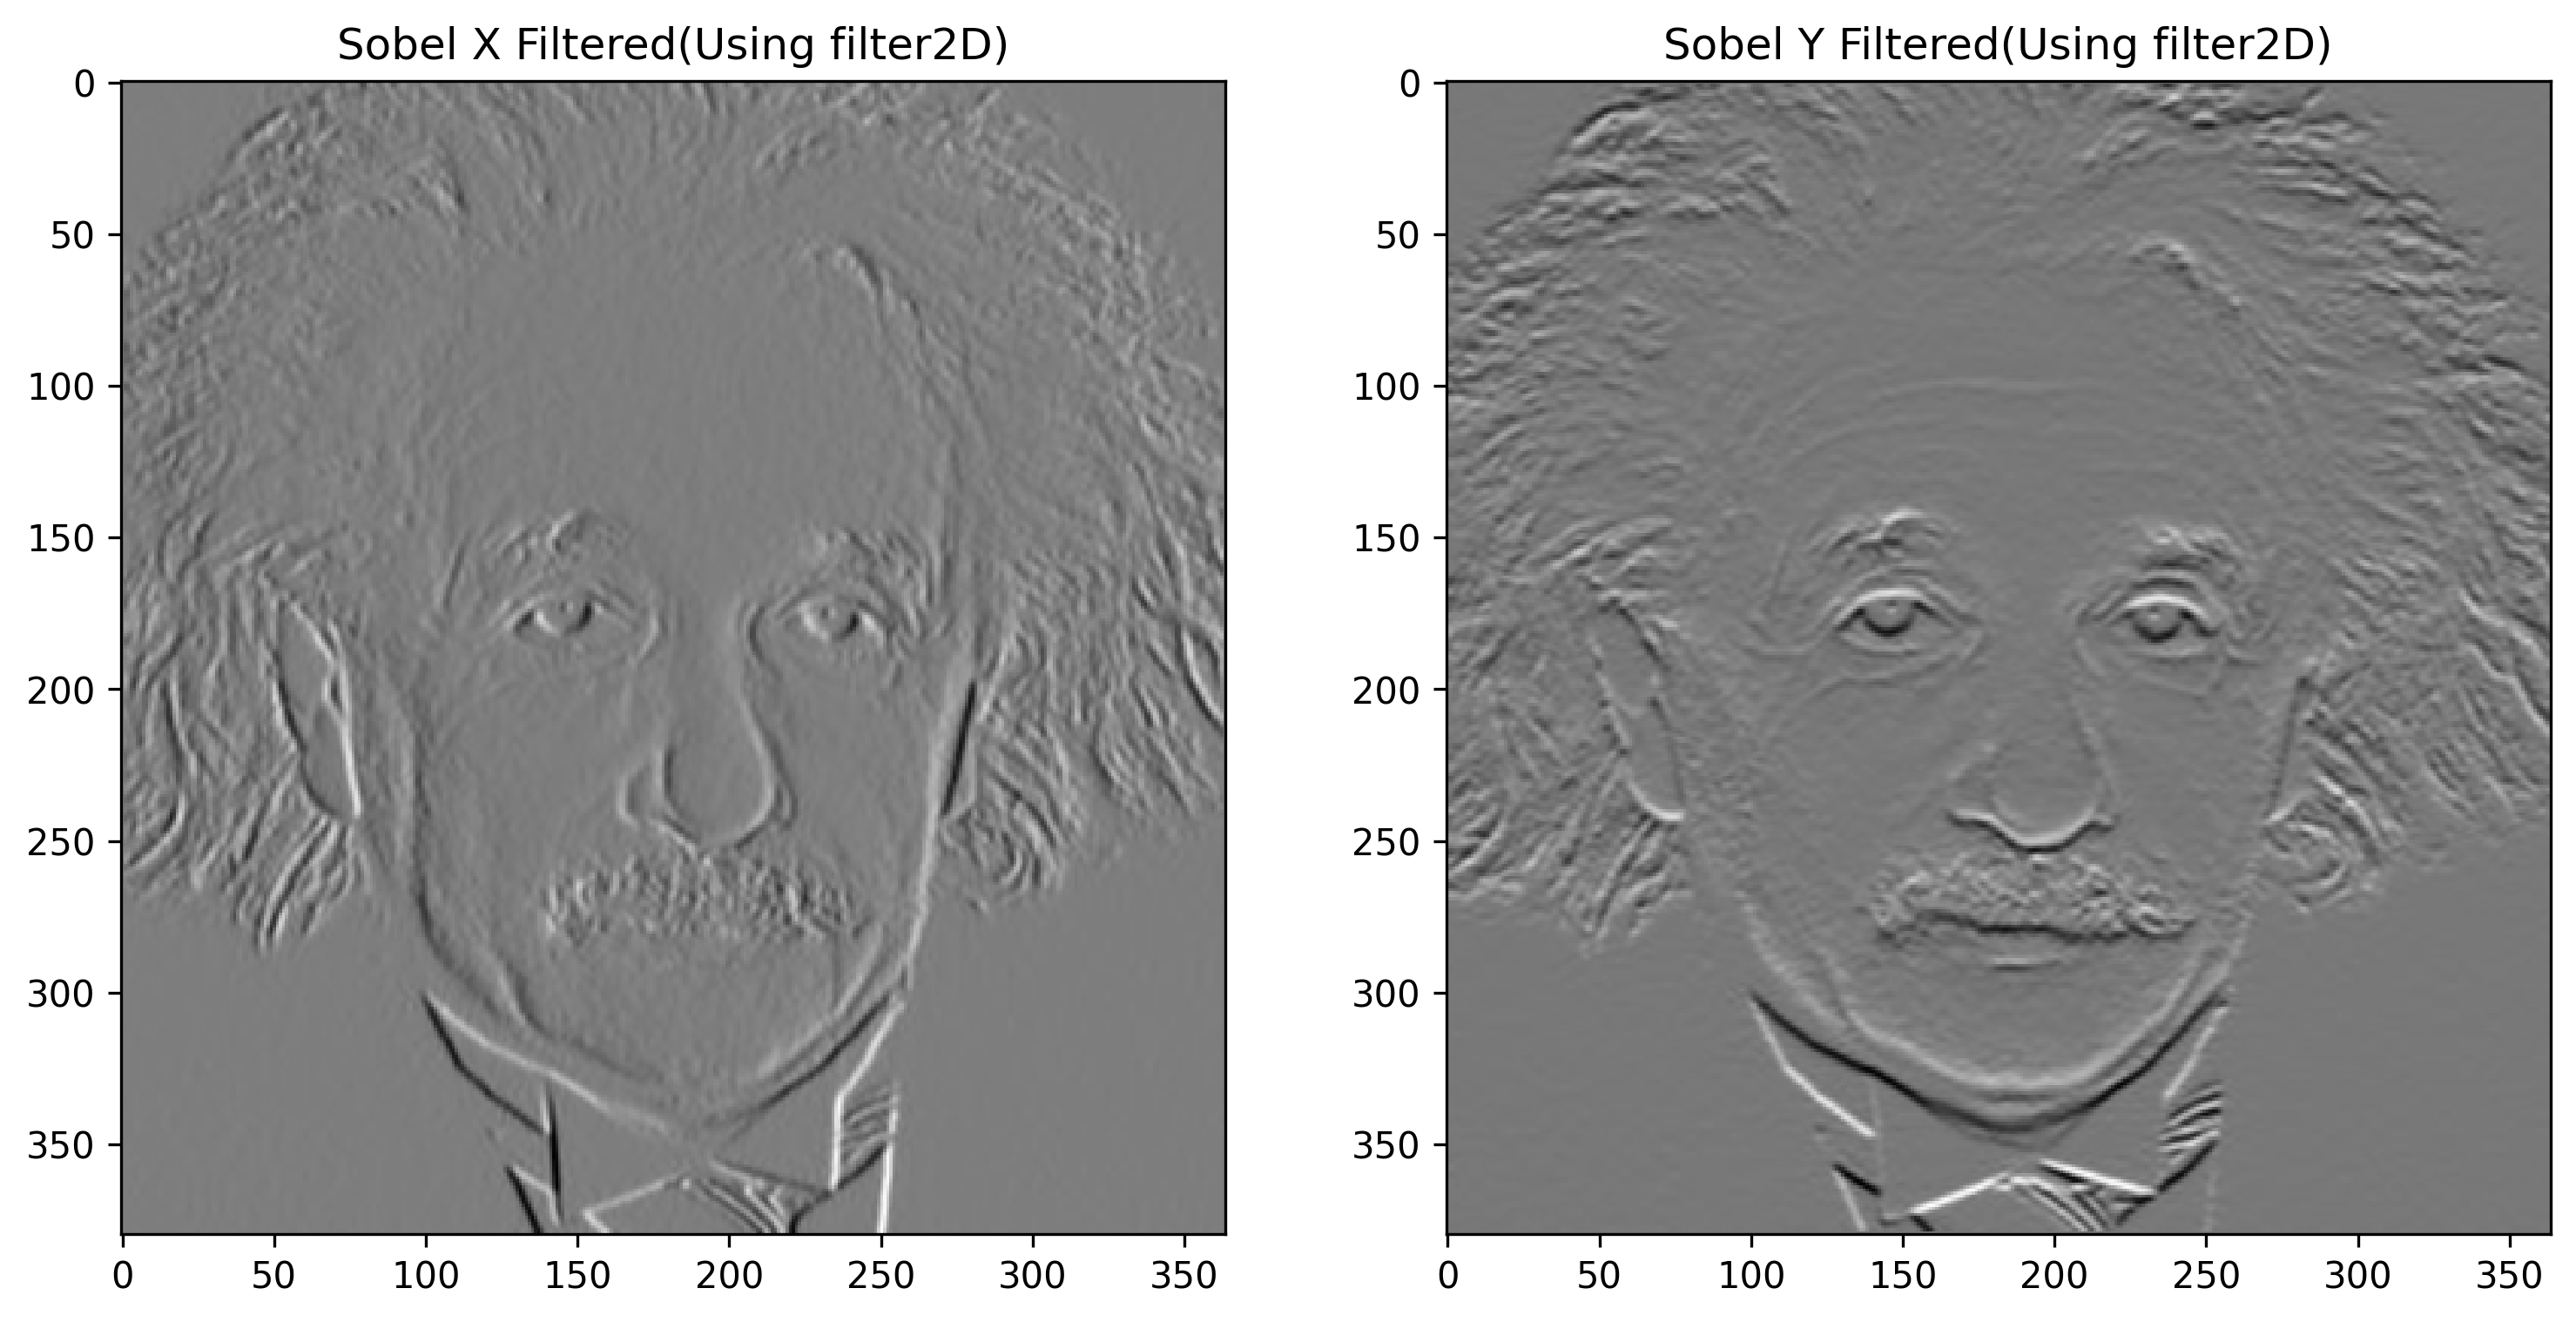
\includegraphics[width=\textwidth]{task7/sobel2D_filtered.png}
        \caption{OpenCV filter2D result}
    \end{subfigure}
    \begin{subfigure}{0.48\textwidth}
        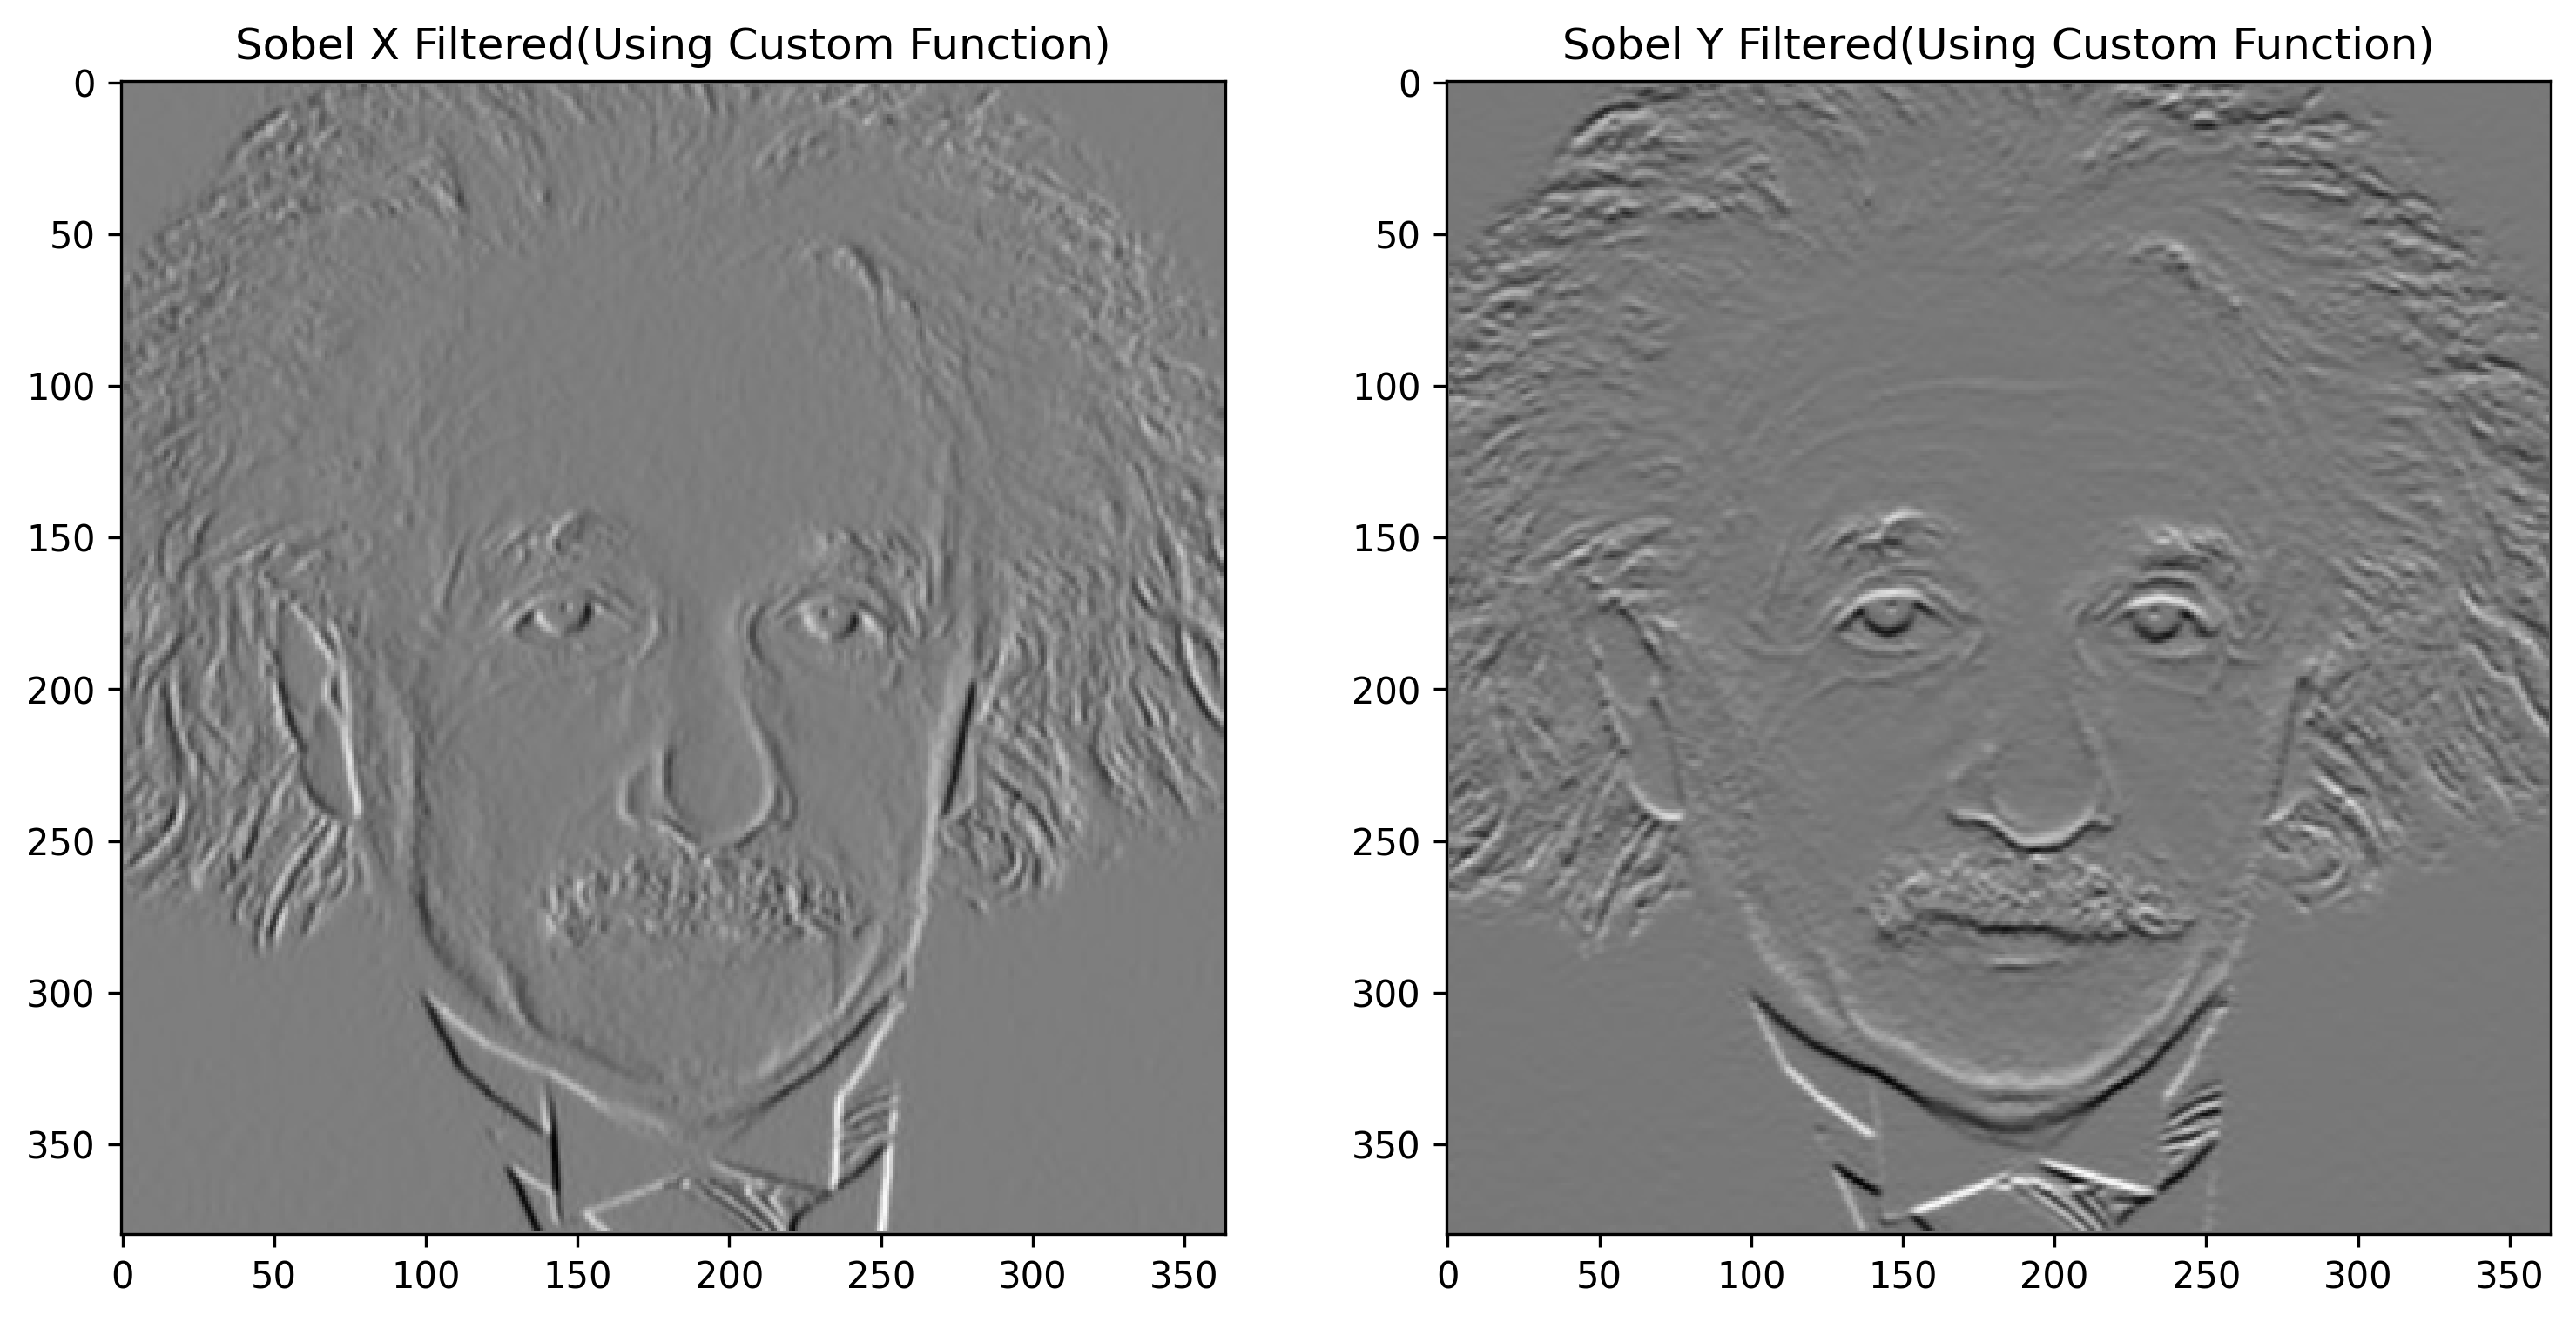
\includegraphics[width=\textwidth]{task7/sobel_custom_filtered.png}
        \caption{Custom implementation}
    \end{subfigure}
    \caption{Sobel filtering comparison}
\end{figure}

\begin{figure}[H]
    \centering
    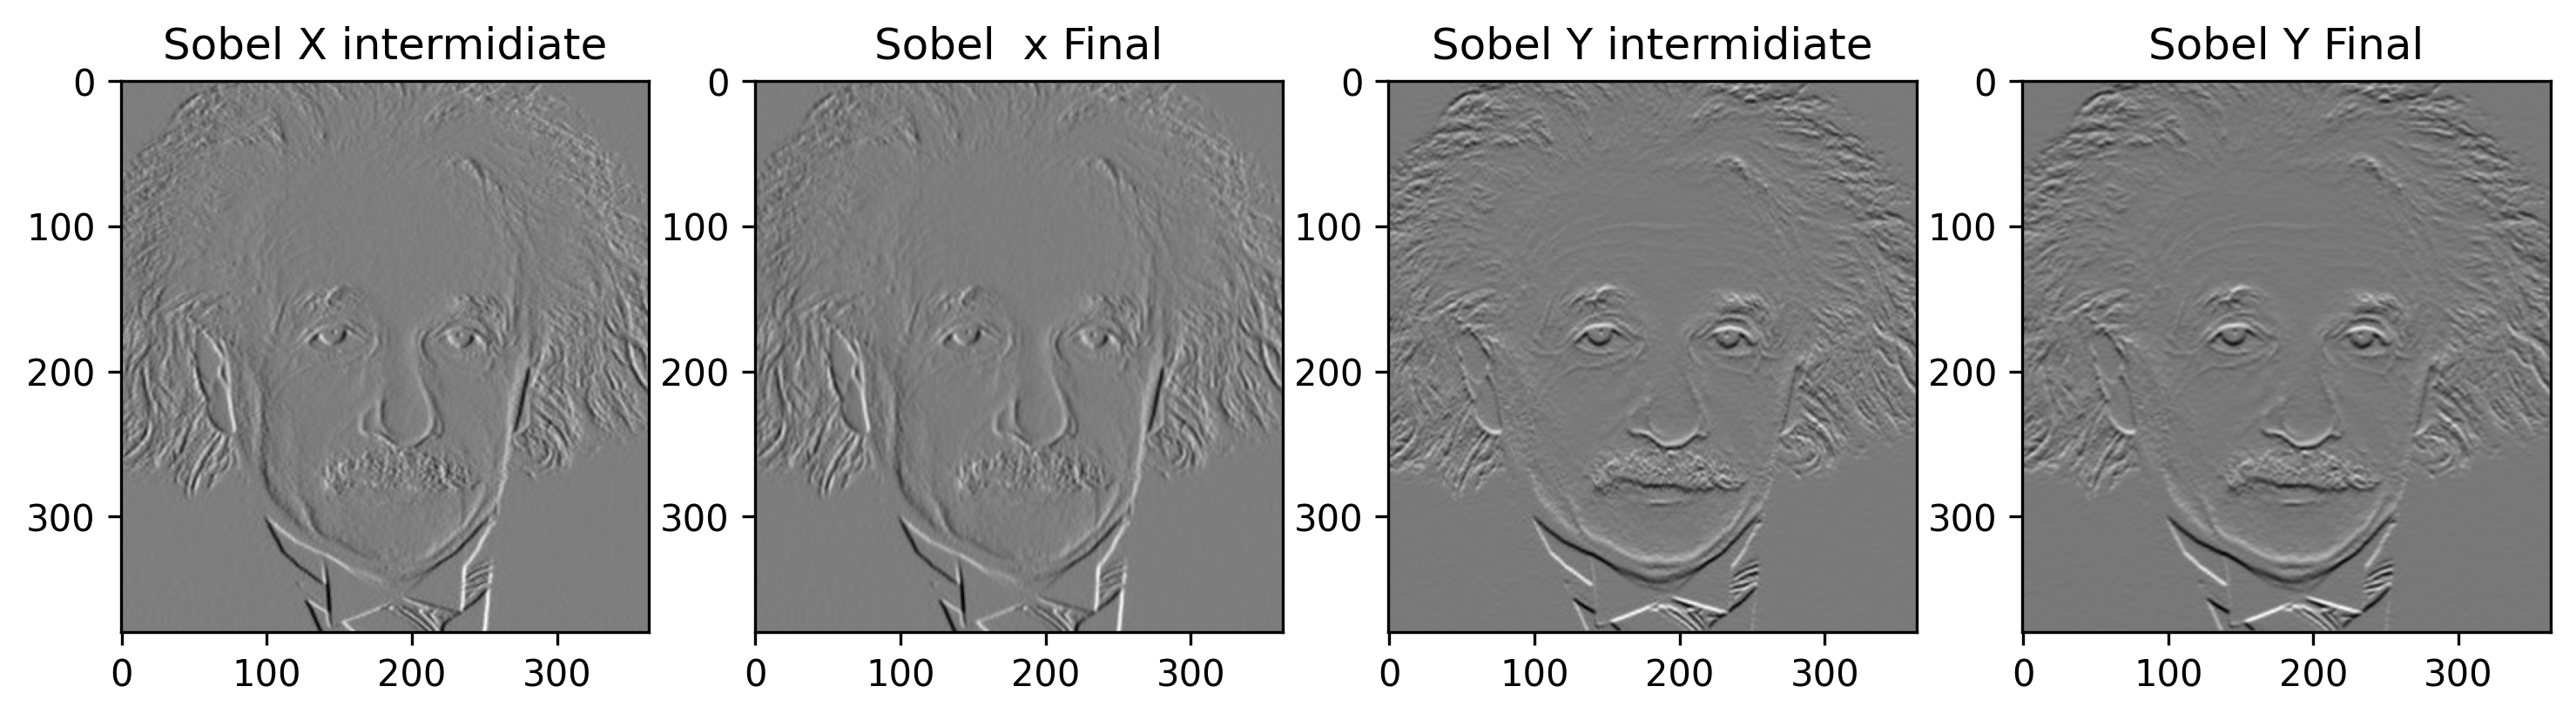
\includegraphics[width=\textwidth]{task7/sobel_combined_filtered.png}
    \caption{Separable convolution}
\end{figure}


\begin{lstlisting}[caption=Custom Sobel filtering implementation]
def sobel_filter(img, filter):
    """Apply Sobel filter to an image."""
    rows, cols = img.shape
    filtered_img = np.zeros_like(img, dtype=np.float64)

    for i in range(1, rows - 1):
        for j in range(1, cols - 1):
            region = img[i - 1 : i + 2, j - 1 : j + 2]
            filtered_img[i, j] = np.sum(region * filter)

    return filtered_img

# Sobel kernels
sobel_x = np.array([[-1, 0, 1], [-2, 0, 2], [-1, 0, 1]])
sobel_y = np.array([[-1, -2, -1], [0, 0, 0], [1, 2, 1]])
# Separable kernels
sobel_x_vertical = np.array([[1], [2], [1]])
sobel_x_horizontal = np.array([[1, 0, -1]])

sobel_y_vertical = np.array([[1], [0], [-1]])
sobel_y_horizontal = np.array([[1, 2, 1]])

x1 = cv.filter2D(einstein, cv.CV_64F, sobel_x_horizontal)
x2 = cv.filter2D(x1, cv.CV_64F, sobel_x_vertical)

y1 = cv.filter2D(einstein, cv.CV_64F, sobel_y_vertical)
y2 = cv.filter2D(y1, cv.CV_64F, sobel_y_horizontal)
\end{lstlisting}

\textbf{Interpretation:} All three approaches produce similar edge detection results, with separable convolution being computationally more efficient.

\section{Question 8}
Image zooming was implemented using both nearest neighbor and bilinear interpolation methods.

\begin{lstlisting}[caption=Image zooming implementation]
# zoom the image with given scale (s)
def zoom_cv(img, s: float, method: str = "nearest"):
    interp = cv.INTER_NEAREST if method == "nearest" else cv.INTER_LINEAR  # bilinear
    h, w = img.shape[:2]
    out = cv.resize(img, None, fx=s, fy=s, interpolation=interp)
    return out

# Calculate normalized SSD for comparison
def normalized_ssd(A, B, max_val=255.0):
    if A.shape == B.shape:
        ssd = np.sum((A - B) ** 2)
        return float(ssd / A.size)
    else:
        print("A and B must have the same shape")
        return None
\end{lstlisting}

\begin{figure}[H]
    \centering
    \begin{subfigure}{0.48\textwidth}
        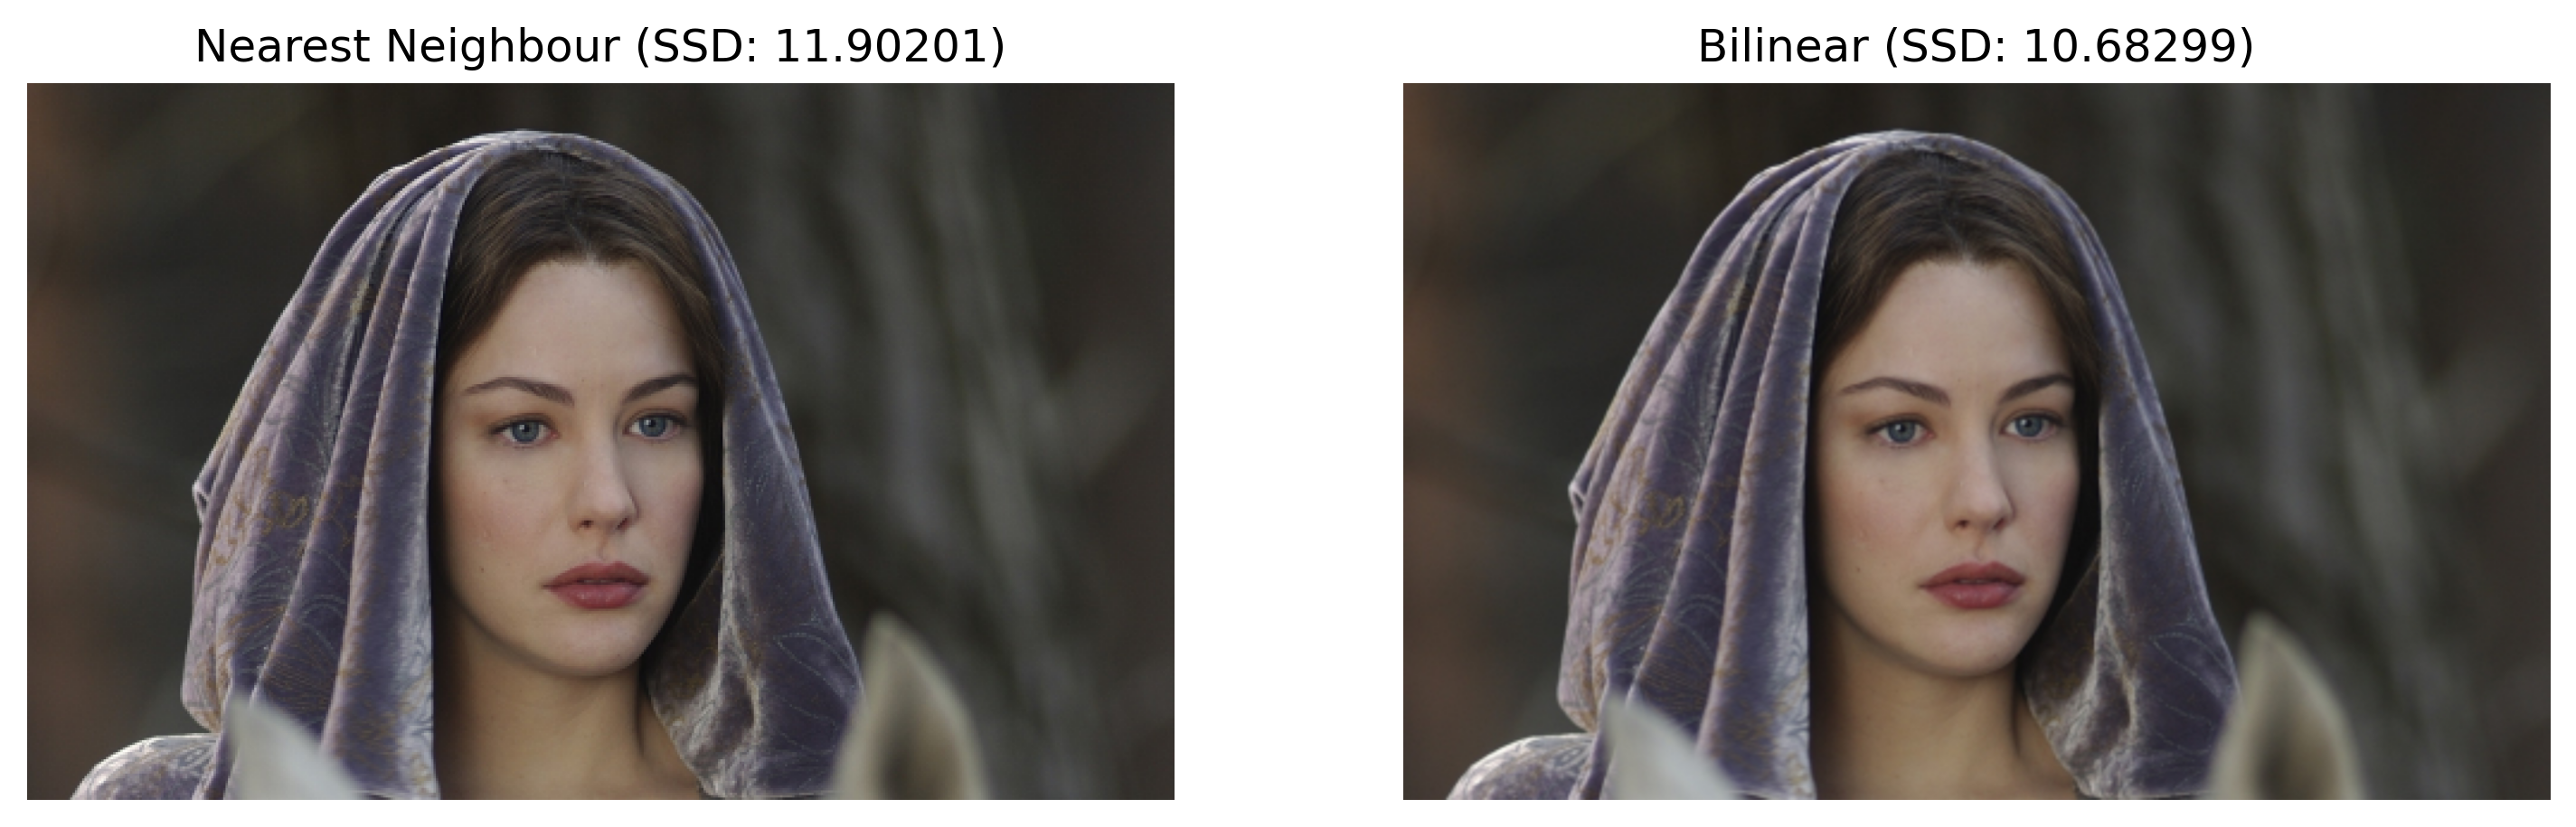
\includegraphics[width=\textwidth]{task8/comparison_nearest_ssd_11_90201.png}
        \caption{Nearest neighbor comparison}
    \end{subfigure}
    \hfill
    \begin{subfigure}{0.48\textwidth}
        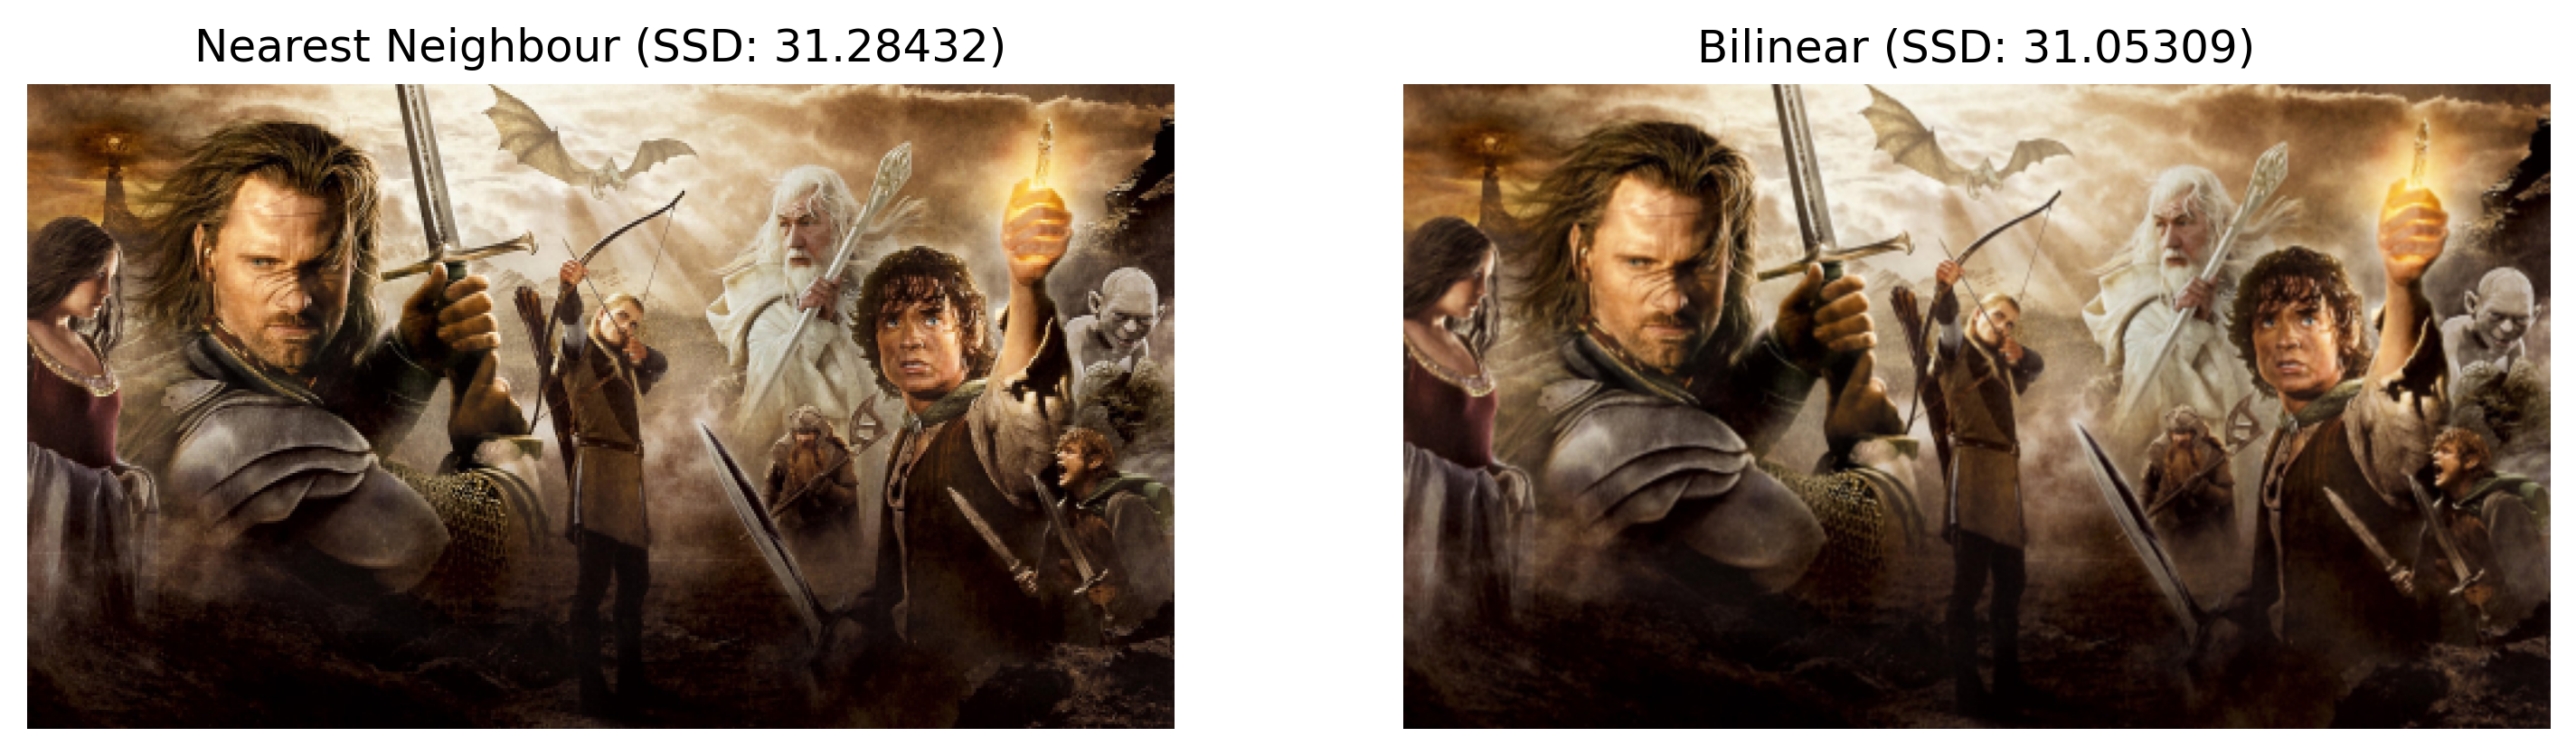
\includegraphics[width=\textwidth]{task8/comparison_nearest_ssd_31_28432.png}
        \caption{Bilinear comparison}
    \end{subfigure}
    \caption{Image zooming results with SSD values}
\end{figure}

\textbf{Interpretation:}Bilinear interpolation produces smoother and more visually pleasing results compared to nearest neighbor. The SSD value is slightly lower for bilinear than for nearest neighbor, indicating a closer match to the reference image.

\newpage

\section{Question 9}
GrabCut algorithm was used for foreground-background segmentation followed by selective background blurring.

\begin{lstlisting}[caption=GrabCut segmentation and background blur]
# GrabCut segmentation
mask = np.zeros(img.shape[:2], np.uint8)
bgdModel = np.zeros((1, 65), np.float64)
fgdModel = np.zeros((1, 65), np.float64)
rect = (50, 100, 550, 550)

cv.grabCut(img, mask, rect, bgdModel, fgdModel, 5, cv.GC_INIT_WITH_RECT)

# Convert mask to binary foreground/background
mask2 = np.where((mask == 2) | (mask == 0), 0, 1).astype("uint8")
foreground = img * mask2[:, :, np.newaxis]
background = img * (1 - mask2[:, :, np.newaxis])

# Blur background
blurred_bg = cv.GaussianBlur(background, (51, 51), 0)
enhanced_img = cv.add(foreground, blurred_bg)

# Convert mask to 3-channel for visualization
mask_vis = cv.cvtColor(mask2 * 255, cv.COLOR_GRAY2BGR)
\end{lstlisting}

\begin{figure}[H]
    \centering
    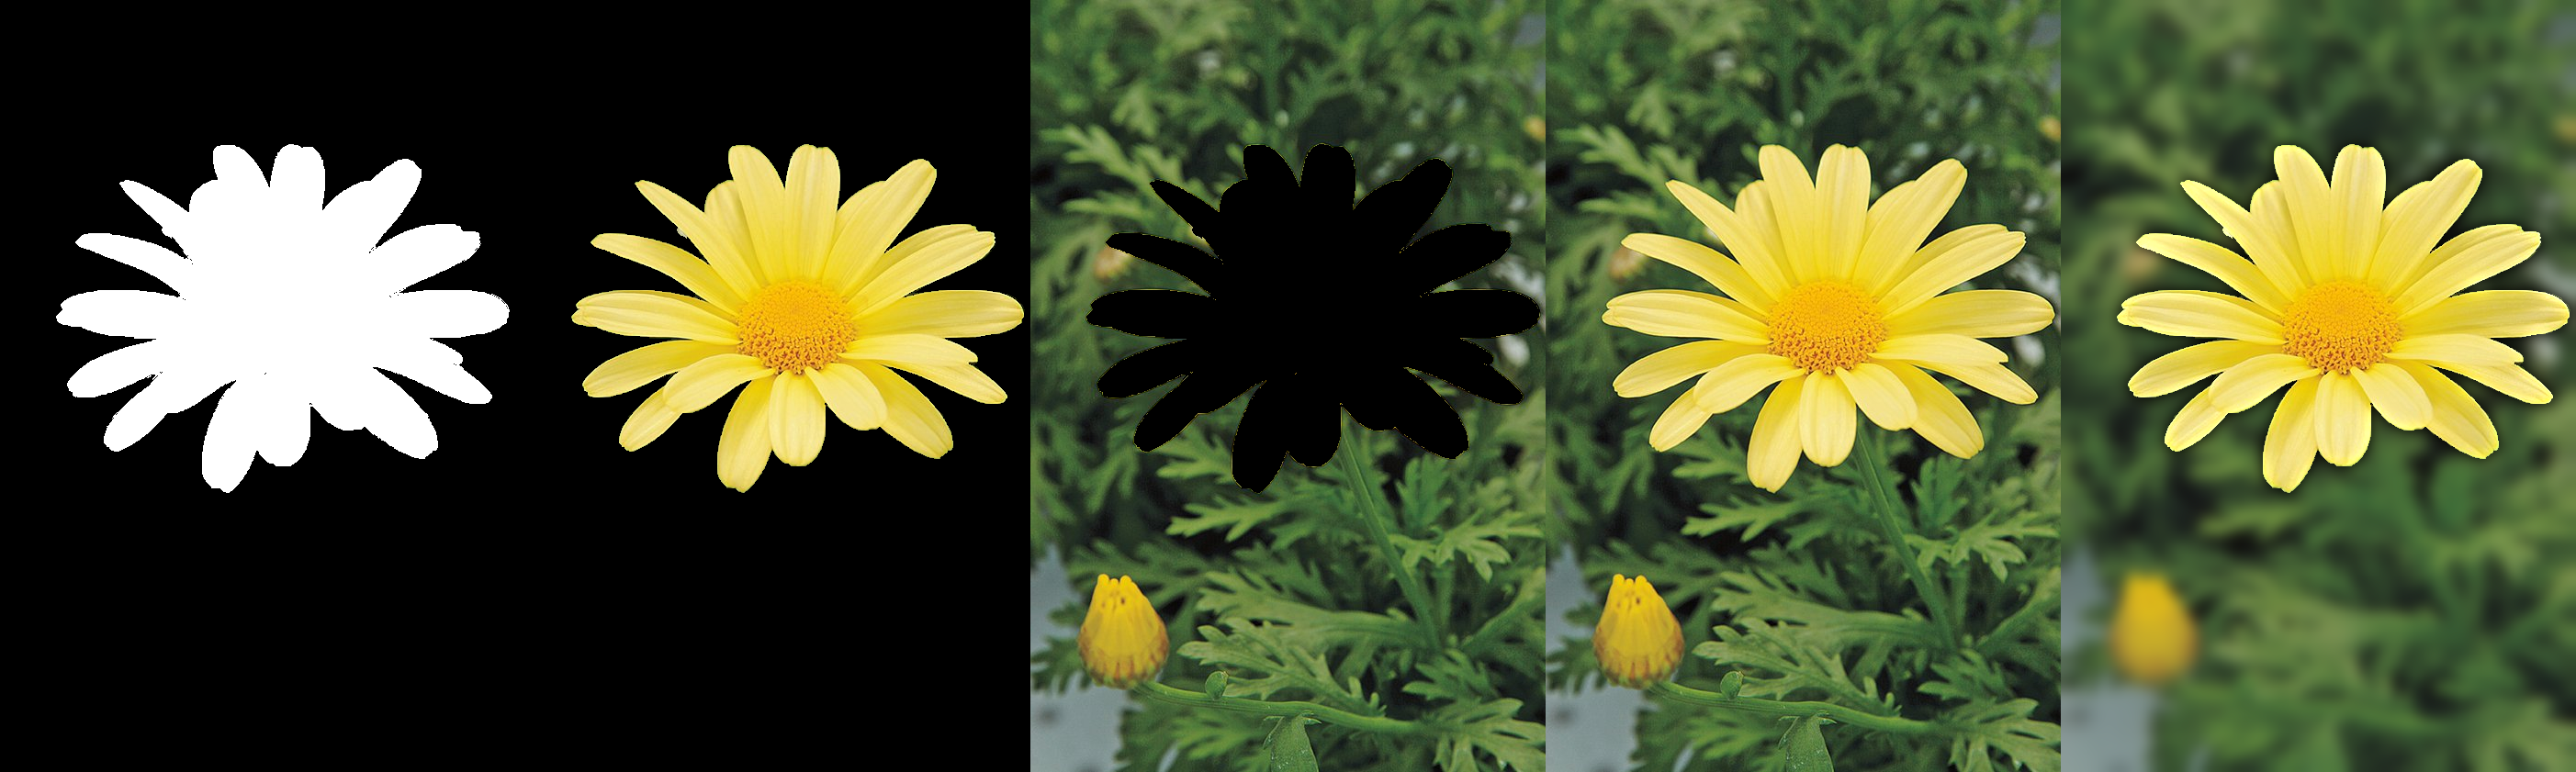
\includegraphics[width=0.8\textwidth]{task9/q9_outputs.png}
    \caption{GrabCut segmentation and background blur results}
\end{figure}

\textbf{Interpretation:} The background appears dark near the flower edges because the Gaussian blur averages neighboring pixels, and pixels replaced by zero (from foreground extraction) contribute to this darkening effect at the boundaries.

\textbf{Reason for dark background at flower edges:} When applying Gaussian blur to the background, the kernel averages surrounding pixels. Near the flower edges, some of these pixels have been set to zero during foreground extraction, causing the averaged values to be darker than the original background pixels.

\end{document}